% Options for packages loaded elsewhere
% Options for packages loaded elsewhere
\PassOptionsToPackage{unicode}{hyperref}
\PassOptionsToPackage{hyphens}{url}
\PassOptionsToPackage{dvipsnames,svgnames,x11names}{xcolor}
%
\documentclass[
  11pt,
  a4paper,
]{article}
\usepackage{xcolor}
\usepackage[margin=1in]{geometry}
\usepackage{amsmath,amssymb}
\setcounter{secnumdepth}{3}
\usepackage{iftex}
\ifPDFTeX
  \usepackage[T1]{fontenc}
  \usepackage[utf8]{inputenc}
  \usepackage{textcomp} % provide euro and other symbols
\else % if luatex or xetex
  \usepackage{unicode-math} % this also loads fontspec
  \defaultfontfeatures{Scale=MatchLowercase}
  \defaultfontfeatures[\rmfamily]{Ligatures=TeX,Scale=1}
\fi
\usepackage{lmodern}
\ifPDFTeX\else
  % xetex/luatex font selection
  \setmainfont[]{Libertinus Serif}
  \setsansfont[]{Jost}
\fi
% Use upquote if available, for straight quotes in verbatim environments
\IfFileExists{upquote.sty}{\usepackage{upquote}}{}
\IfFileExists{microtype.sty}{% use microtype if available
  \usepackage[]{microtype}
  \UseMicrotypeSet[protrusion]{basicmath} % disable protrusion for tt fonts
}{}
\makeatletter
\@ifundefined{KOMAClassName}{% if non-KOMA class
  \IfFileExists{parskip.sty}{%
    \usepackage{parskip}
  }{% else
    \setlength{\parindent}{0pt}
    \setlength{\parskip}{6pt plus 2pt minus 1pt}}
}{% if KOMA class
  \KOMAoptions{parskip=half}}
\makeatother

\usepackage{color}
\usepackage{fancyvrb}
\newcommand{\VerbBar}{|}
\newcommand{\VERB}{\Verb[commandchars=\\\{\}]}
\DefineVerbatimEnvironment{Highlighting}{Verbatim}{commandchars=\\\{\}}
% Add ',fontsize=\small' for more characters per line
\usepackage{framed}
\definecolor{shadecolor}{RGB}{241,243,245}
\newenvironment{Shaded}{\begin{snugshade}}{\end{snugshade}}
\newcommand{\AlertTok}[1]{\textcolor[rgb]{0.68,0.00,0.00}{#1}}
\newcommand{\AnnotationTok}[1]{\textcolor[rgb]{0.37,0.37,0.37}{#1}}
\newcommand{\AttributeTok}[1]{\textcolor[rgb]{0.40,0.45,0.13}{#1}}
\newcommand{\BaseNTok}[1]{\textcolor[rgb]{0.68,0.00,0.00}{#1}}
\newcommand{\BuiltInTok}[1]{\textcolor[rgb]{0.00,0.23,0.31}{#1}}
\newcommand{\CharTok}[1]{\textcolor[rgb]{0.13,0.47,0.30}{#1}}
\newcommand{\CommentTok}[1]{\textcolor[rgb]{0.37,0.37,0.37}{#1}}
\newcommand{\CommentVarTok}[1]{\textcolor[rgb]{0.37,0.37,0.37}{\textit{#1}}}
\newcommand{\ConstantTok}[1]{\textcolor[rgb]{0.56,0.35,0.01}{#1}}
\newcommand{\ControlFlowTok}[1]{\textcolor[rgb]{0.00,0.23,0.31}{\textbf{#1}}}
\newcommand{\DataTypeTok}[1]{\textcolor[rgb]{0.68,0.00,0.00}{#1}}
\newcommand{\DecValTok}[1]{\textcolor[rgb]{0.68,0.00,0.00}{#1}}
\newcommand{\DocumentationTok}[1]{\textcolor[rgb]{0.37,0.37,0.37}{\textit{#1}}}
\newcommand{\ErrorTok}[1]{\textcolor[rgb]{0.68,0.00,0.00}{#1}}
\newcommand{\ExtensionTok}[1]{\textcolor[rgb]{0.00,0.23,0.31}{#1}}
\newcommand{\FloatTok}[1]{\textcolor[rgb]{0.68,0.00,0.00}{#1}}
\newcommand{\FunctionTok}[1]{\textcolor[rgb]{0.28,0.35,0.67}{#1}}
\newcommand{\ImportTok}[1]{\textcolor[rgb]{0.00,0.46,0.62}{#1}}
\newcommand{\InformationTok}[1]{\textcolor[rgb]{0.37,0.37,0.37}{#1}}
\newcommand{\KeywordTok}[1]{\textcolor[rgb]{0.00,0.23,0.31}{\textbf{#1}}}
\newcommand{\NormalTok}[1]{\textcolor[rgb]{0.00,0.23,0.31}{#1}}
\newcommand{\OperatorTok}[1]{\textcolor[rgb]{0.37,0.37,0.37}{#1}}
\newcommand{\OtherTok}[1]{\textcolor[rgb]{0.00,0.23,0.31}{#1}}
\newcommand{\PreprocessorTok}[1]{\textcolor[rgb]{0.68,0.00,0.00}{#1}}
\newcommand{\RegionMarkerTok}[1]{\textcolor[rgb]{0.00,0.23,0.31}{#1}}
\newcommand{\SpecialCharTok}[1]{\textcolor[rgb]{0.37,0.37,0.37}{#1}}
\newcommand{\SpecialStringTok}[1]{\textcolor[rgb]{0.13,0.47,0.30}{#1}}
\newcommand{\StringTok}[1]{\textcolor[rgb]{0.13,0.47,0.30}{#1}}
\newcommand{\VariableTok}[1]{\textcolor[rgb]{0.07,0.07,0.07}{#1}}
\newcommand{\VerbatimStringTok}[1]{\textcolor[rgb]{0.13,0.47,0.30}{#1}}
\newcommand{\WarningTok}[1]{\textcolor[rgb]{0.37,0.37,0.37}{\textit{#1}}}

\usepackage{longtable,booktabs,array}
\newcounter{none} % for unnumbered tables
\usepackage{calc} % for calculating minipage widths
% Correct order of tables after \paragraph or \subparagraph
\usepackage{etoolbox}
\makeatletter
\patchcmd\longtable{\par}{\if@noskipsec\mbox{}\fi\par}{}{}
\makeatother
% Allow footnotes in longtable head/foot
\IfFileExists{footnotehyper.sty}{\usepackage{footnotehyper}}{\usepackage{footnote}}
\makesavenoteenv{longtable}
\usepackage{graphicx}
\makeatletter
\newsavebox\pandoc@box
\newcommand*\pandocbounded[1]{% scales image to fit in text height/width
  \sbox\pandoc@box{#1}%
  \Gscale@div\@tempa{\textheight}{\dimexpr\ht\pandoc@box+\dp\pandoc@box\relax}%
  \Gscale@div\@tempb{\linewidth}{\wd\pandoc@box}%
  \ifdim\@tempb\p@<\@tempa\p@\let\@tempa\@tempb\fi% select the smaller of both
  \ifdim\@tempa\p@<\p@\scalebox{\@tempa}{\usebox\pandoc@box}%
  \else\usebox{\pandoc@box}%
  \fi%
}
% Set default figure placement to htbp
\def\fps@figure{htbp}
\makeatother


% definitions for citeproc citations
\NewDocumentCommand\citeproctext{}{}
\NewDocumentCommand\citeproc{mm}{%
  \begingroup\def\citeproctext{#2}\cite{#1}\endgroup}
\makeatletter
 % allow citations to break across lines
 \let\@cite@ofmt\@firstofone
 % avoid brackets around text for \cite:
 \def\@biblabel#1{}
 \def\@cite#1#2{{#1\if@tempswa , #2\fi}}
\makeatother
\newlength{\cslhangindent}
\setlength{\cslhangindent}{1.5em}
\newlength{\csllabelwidth}
\setlength{\csllabelwidth}{3em}
\newenvironment{CSLReferences}[2] % #1 hanging-indent, #2 entry-spacing
 {\begin{list}{}{%
  \setlength{\itemindent}{0pt}
  \setlength{\leftmargin}{0pt}
  \setlength{\parsep}{0pt}
  % turn on hanging indent if param 1 is 1
  \ifodd #1
   \setlength{\leftmargin}{\cslhangindent}
   \setlength{\itemindent}{-1\cslhangindent}
  \fi
  % set entry spacing
  \setlength{\itemsep}{#2\baselineskip}}}
 {\end{list}}
\usepackage{calc}
\newcommand{\CSLBlock}[1]{\hfill\break\parbox[t]{\linewidth}{\strut\ignorespaces#1\strut}}
\newcommand{\CSLLeftMargin}[1]{\parbox[t]{\csllabelwidth}{\strut#1\strut}}
\newcommand{\CSLRightInline}[1]{\parbox[t]{\linewidth - \csllabelwidth}{\strut#1\strut}}
\newcommand{\CSLIndent}[1]{\hspace{\cslhangindent}#1}



\setlength{\emergencystretch}{3em} % prevent overfull lines

\providecommand{\tightlist}{%
  \setlength{\itemsep}{0pt}\setlength{\parskip}{0pt}}



 


% -----------------------
% CUSTOM PREAMBLE STUFF
% -----------------------

% -----------------
% Title block stuff
% -----------------

% Abstract
\usepackage[runin]{abstract}
\renewcommand{\abstractnamefont}{\sffamily\small\bfseries}
\renewcommand{\abstracttextfont}{\sffamily\small}
\setlength{\absleftindent}{5pt}
\setlength{\absrightindent}{\absleftindent}

% Title
\usepackage{titling}
\pretitle{\par\begin{flushleft}\LARGE\sffamily\bfseries}
\posttitle{\par\end{flushleft}\vskip 10pt}

% Keywords
\newenvironment{keywords}
{\small\sffamily{\sffamily\small\bfseries{Keywords.}}}

% Authors
\usepackage{orcidlink}  % Create automatic ORCID icons/links
%\renewcommand{\and}{\end{tabular} \hskip 3em \begin{tabular}[t]{@{\hspace{0em}}l@{}}}
\preauthor{\begin{flushleft}
           \lineskip 1.5em}
\postauthor{\end{flushleft}}

% ------------------
% Section headings
% ------------------
\usepackage{titlesec}
\titleformat*{\section}{\Large\sffamily\bfseries\raggedright}
\titleformat*{\subsection}{\large\sffamily\bfseries\raggedright}
\titleformat*{\subsubsection}{\normalsize\sffamily\bfseries\raggedright}
\titleformat*{\paragraph}{\small\sffamily\bfseries\raggedright}

%\titlespacing{<command>}{<left>}{<before-sep>}{<after-sep>}
% Starred version removes indentation in following paragraph
\titlespacing*{\section}{0em}{2em}{0.1em}
\titlespacing*{\subsection}{0em}{1.25em}{0.1em}
\titlespacing*{\subsubsection}{0em}{0.75em}{0em}

% ------------------
% Headers/Footers
% ------------------
\usepackage{fancyhdr}
\pagestyle{fancy}
\fancyhf{}
\fancyhead[L,C,R]{}
\fancyfoot[L,C]{}
\fancyfoot[R]{\thepage}
\renewcommand{\headrulewidth}{1pt}
\fancypagestyle{plain}{%
    \renewcommand{\headrulewidth}{0pt}%
    \fancyhf{}%
    \fancyfoot[R]{\thepage}%
}
\renewcommand\footnoterule{\rule{\linewidth}{0.1pt}\vspace{5pt}}

% ------------------
% Captions
% ------------------
\usepackage[labelfont=bf,labelsep=period]{caption}
\captionsetup[figure]{font=footnotesize,justification=raggedright,singlelinecheck=false,format=hang}


% ---------------------------
% END CUSTOM PREAMBLE STUFF
% ---------------------------
\usepackage{float}
\usepackage{tabularray}
\usepackage[normalem]{ulem}
\usepackage{graphicx}
\usepackage{rotating}
\UseTblrLibrary{siunitx}
\NewTableCommand{\tinytableDefineColor}[3]{\definecolor{#1}{#2}{#3}}
\newcommand{\tinytableTabularrayUnderline}[1]{\underline{#1}}
\newcommand{\tinytableTabularrayStrikeout}[1]{\sout{#1}}
\newcommand{\pkg}[1]{{\fontseries{b}\selectfont #1}}
\usepackage[utf8]{inputenc}
\usepackage{amsmath}
\usepackage{amsfonts}
\usepackage{mathtools}
\usepackage{pdflscape}
\usepackage{xcolor}
\usepackage{booktabs, caption, longtable, colortbl, array}
\usepackage[font=small,labelfont={bf,small}]{caption}
\usepackage{multirow}
\usepackage{wrapfig}
\usepackage{float}
\usepackage{pdflscape}
\usepackage{tabu}
\usepackage{threeparttable}
\usepackage{threeparttablex}
\usepackage[normalem]{ulem}
\usepackage{makecell}
\newcommand{\blandscape}{\begin{landscape}}
\newcommand{\elandscape}{\end{landscape}}
\usepackage{underscore}
\usepackage{fancyvrb}

\makeatletter
\@ifpackageloaded{tcolorbox}{}{\usepackage[skins,breakable]{tcolorbox}}
\@ifpackageloaded{fontawesome5}{}{\usepackage{fontawesome5}}
\definecolor{quarto-callout-color}{HTML}{909090}
\definecolor{quarto-callout-note-color}{HTML}{0758E5}
\definecolor{quarto-callout-important-color}{HTML}{CC1914}
\definecolor{quarto-callout-warning-color}{HTML}{EB9113}
\definecolor{quarto-callout-tip-color}{HTML}{00A047}
\definecolor{quarto-callout-caution-color}{HTML}{FC5300}
\definecolor{quarto-callout-color-frame}{HTML}{acacac}
\definecolor{quarto-callout-note-color-frame}{HTML}{4582ec}
\definecolor{quarto-callout-important-color-frame}{HTML}{d9534f}
\definecolor{quarto-callout-warning-color-frame}{HTML}{f0ad4e}
\definecolor{quarto-callout-tip-color-frame}{HTML}{02b875}
\definecolor{quarto-callout-caution-color-frame}{HTML}{fd7e14}
\makeatother
\makeatletter
\@ifpackageloaded{caption}{}{\usepackage{caption}}
\AtBeginDocument{%
\ifdefined\contentsname
  \renewcommand*\contentsname{Table of contents}
\else
  \newcommand\contentsname{Table of contents}
\fi
\ifdefined\listfigurename
  \renewcommand*\listfigurename{List of Figures}
\else
  \newcommand\listfigurename{List of Figures}
\fi
\ifdefined\listtablename
  \renewcommand*\listtablename{List of Tables}
\else
  \newcommand\listtablename{List of Tables}
\fi
\ifdefined\figurename
  \renewcommand*\figurename{Figure}
\else
  \newcommand\figurename{Figure}
\fi
\ifdefined\tablename
  \renewcommand*\tablename{Table}
\else
  \newcommand\tablename{Table}
\fi
}
\@ifpackageloaded{float}{}{\usepackage{float}}
\floatstyle{ruled}
\@ifundefined{c@chapter}{\newfloat{codelisting}{h}{lop}}{\newfloat{codelisting}{h}{lop}[chapter]}
\floatname{codelisting}{Listing}
\newcommand*\listoflistings{\listof{codelisting}{List of Listings}}
\makeatother
\makeatletter
\makeatother
\makeatletter
\@ifpackageloaded{caption}{}{\usepackage{caption}}
\@ifpackageloaded{subcaption}{}{\usepackage{subcaption}}
\makeatother
\usepackage{bookmark}
\IfFileExists{xurl.sty}{\usepackage{xurl}}{} % add URL line breaks if available
\urlstyle{same}
\hypersetup{
  pdftitle={: an R package for mathematically aggregating expert judgements},
  pdfauthor={Elliot Gould; Charles T. Gray; Aaron Willcox; Rose E. O'Dea; Rebecca Groenewegen; David P. Wilkinson},
  pdfkeywords={mathematical aggregation, expert
judgement, replicability, R},
  colorlinks=true,
  linkcolor={blue},
  filecolor={Maroon},
  citecolor={Blue},
  urlcolor={blue},
  pdfcreator={LaTeX via pandoc}}



\title{\pkg{aggreCAT}: an R package for mathematically aggregating
expert judgements}
% subtitles do not seem to work with article class?
%%\subtitle{}

\author{
{\bfseries \normalsize Elliot Gould~\orcidlink{0000-0002-6585-538X}}%
 \\%
 \small School of Agriculture, Food and Ecosystem Sciences, The
University of Melbourne \\ \small School of Historical and Philosophical
Studies, The University of Melbourne \\%
{\footnotesize \nolinkurl{elliot.gould@unimelb.edu.au}} \\\vspace{10pt}
{\bfseries \normalsize Charles T. Gray}%
 \\%
 \small Evidence Synthesis Lab, Newcastle University \\%
{\footnotesize \nolinkurl{}} \\\vspace{10pt}
{\bfseries \normalsize Aaron Willcox~\orcidlink{0000-0003-2536-2596}}%
 \\%
 \small School of Historical and Philosophical Studies, The University
of Melbourne \\%
{\footnotesize \nolinkurl{}} \\\vspace{10pt}
{\bfseries \normalsize Rose E. O'Dea~\orcidlink{0000-0001-8177-5075}}%
 \\%
 \small School of Historical and Philosophical Studies, The University
of Melbourne \\%
{\footnotesize \nolinkurl{}} \\\vspace{10pt}
{\bfseries \normalsize Rebecca
Groenewegen~\orcidlink{0000-0001-9177-8536}}%
 \\%
 \small School of Agriculture, Food and Ecosystem Sciences, The
University of Melbourne \\%
{\footnotesize \nolinkurl{}} \\\vspace{10pt}
{\bfseries \normalsize David P.
Wilkinson~\orcidlink{0000-0002-9560-6499}}%
 \\%
 \small School of Agriculture, Food and Ecosystem Sciences, The
University of Melbourne \\%
{\footnotesize \nolinkurl{}} \\\vspace{10pt}
}

\predate{}
\postdate{}
\date{}
\begin{document}

% for some reason this does not work in header
\renewcommand{\abstractname}{Abstract.}

% add the short title to the fancy header

\maketitle
%\noindent \rule{\linewidth}{.5pt}
\begin{abstract}
Structured elicitation protocols, such as the IDEA protocol, are used to
elicit probabilistic judgements from multiple domain experts about
uncertain events across fields including ecology, biosecurity risk
assessment, and metascience. Individual expert judgements must
subsequently be mathematically aggregated into a single group forecast.
While the simplest case involves combining a set of point-estimates from
multiple individuals, this process is further complicated when
judgements include uncertainty bounds, or when elicitation is conducted
across multiple rounds. This paper presents \pkg{aggreCAT}, an
open-source \proglang{R} package that provides 29 aggregation methods
for combining individual expert judgements into a single probabilistic
estimate, accommodating designs ranging from single-round point
estimates to multi-round three-point elicitation. The package follows
tidy data principles, enabling straightforward integration with existing
R workflows for application at scale. Methods range from unweighted
arithmetic combinations to performance-weighted schemes and Bayesian
models, with weights derived from uncertainty intervals, shifts in
judgements between elicitation rounds, and breadth of expert reasoning.
We provide worked examples illustrating the mechanics of representative
aggregation methods, a general workflow for batch aggregation across
multiple forecasts and methods, and built-in functions for evaluating
and visualising forecast performance against known outcomes.
\pkg{aggreCAT} fills a substantive gap in open software for
mathematically aggregating expert judgement, and is intended to support
researchers and decision analysts in rapidly and rigorously synthesising
outputs from structured elicitation exercises.
\end{abstract}
\begin{keywords}
\def\sep{;\ }
mathematical aggregation\sep expert judgement\sep replicability\sep 
R
\end{keywords}
%\noindent \rule{\linewidth}{.5pt}


\section{Introduction}\label{sec-introduction}

Expert judgement is frequently used to inform forecasting about
uncertain future events across a range of fields and applications
including ecological management and decision making (Legge et al. 2022),
biosecurity risk analyses (Wittmann et al. 2015), replicability
forecasts (Mody et al. 2026), and horizon scanning exercises (Sutherland
et al. 2017). Judgements from groups of experts tend to perform better
than a single expert (Goossens et al. 2008), and it is best-practice to
elicit judgements from diverse groups so that group members can bring
``different perspectives, cross-examine each others' reasoning, and
share information'', however judgements or forecasts must then be
distilled into a single forecast, ideally accompanied by estimates of
uncertainty around those estimates ({Hanea et al.} 2021). Judgements
from multiple experts may be combined into a single score using either
behavioural approaches that force experts into forming consensus, or by
using mathematical approaches (Goossens et al. 2008).

Aggregated elicited judgements form a critical component of
decision-making across multiple contexts, and while there are a variety
of methods for mathematically aggregating expert judgements into single
point-predictions, there has been a dearth of accessible tools for
implementing any aggregation more complex than linear averages. Many
existing software tools are closed-source, are irreproducible, or
written in programming languages rarely used by ecologists or
metascientists. Methods implemented in \proglang{R}, one of the most
widely used programming languages in the life sciences (Gao et al.
2025), are limited in scope, or have been archived from CRAN. The
\proglang{R} package \pkg{SHELF} implements only a single method
(weighted linear pool) for aggregating expert judgements (Oakley 2026),
but integrates with \pkg{expertsurv} to incorporate expert judgement
into survival analysis (Cooney and White 2023), while \pkg{opera}
provides a suite of methods for aggregating time-series predictions, but
does not implement methods for aggregating point-predictions with
uncertainty bounds (Gaillard and Goude 2026).

\pkg{aggreCAT} is an open, reliable, and modular R package for the
mathematical aggregation of expert elicitation data with a
straightforward user interface. The \pkg{aggreCAT} package was developed
by the by the repliCATS (Collaborative Assessment for Trustworthy
Science) project (Fraser et al. 2023) as part of the DARPA SCORE
(Systematizing Confidence in Open Research and Evidence) program
(Alipourfard et al. 2021), which aimed to generate quantitative
`confidence scores' --- estimates of the likely replicability of
research claims from the social and behavioural sciences --- for use as
a proxy measure of credibility in the absence of direct replication
effort. \pkg{aggreCAT} arose from the need for a software solution to
reliably conduct mathematical aggregation at scale. The repliCATS
project used \pkg{aggreCAT} to aggregate expert elicited judgements into
confidence scores for \(> 4000\) claims (Mody et al. 2026). While
originally a bespoke implementation for repliCATS, we have since
developed \pkg{aggreCAT} into a more general R package that can handle
most types of elicitation data requiring mathematical aggregation,
allowing for wider applicability.

\pkg{aggreCAT} provides a suite of 29 aggregation methods that explore
different approaches to mathematical aggregation from straightforward
arithmetic calculations to Bayesian statistical models. In addition, we
provide extra functionality such as plotting functions and performance
evaluation against known outcomes. While the repliCATS project uses the
IDEA protocol to structure the elicitation process (Hemming et al.
2017), we have generalised \pkg{aggreCAT} to work with a variety of
elicitation protocols. \pkg{aggreCAT} fills a large void in open
software for aggregating elicited judgements, providing enormous benefit
to researchers and decision makers across any field of research.

In this paper we give an overview of the \pkg{aggreCAT} package so that
researchers may apply any of the the aggregation functions described in
({Hanea et al.} 2021), as well as additional methods provided by
\pkg{aggreCAT}, to their own expert elicitation datasets where
mathematical aggregation is required.

\section{Mathematically aggregating expert
judgements}\label{mathematically-aggregating-expert-judgements}

The aggregation methods in \pkg{aggreCAT} were developed in the context
of the IDEA protocol (Box
\hyperref[box-1-the-replicats-idea-protocol]{1}), a structured
elicitation procedure that draws on the `wisdom of crowds' to elicit
probabilistic judgements from groups of experts about uncertain events.

This elicitation structure directly determines which aggregation methods
in \pkg{aggreCAT} are applicable to a given dataset: most methods
require only the post-discussion (\emph{Round 2}) single-point
judgements, some additionally use the pre-discussion (\emph{Round 1})
judgements, and a small number require supplementary ratings or
externally collected data. These requirements are summarised for each
method in Table~\ref{tbl-method-summary-table}.

Although the aggregation methods were developed in the context of the
IDEA protocol, all methods requiring only a single round of elicitation
can be applied to any structured elicitation procedure, including those
that include multiple rounds of elicitation, or that elicit three-point
estimates without enforcing behavioural consensus.

\begin{tcolorbox}[enhanced jigsaw, arc=.35mm, bottomrule=.15mm, breakable, colback=white, colframe=quarto-callout-color-frame, left=2mm, leftrule=.75mm, opacityback=0, rightrule=.15mm, toprule=.15mm]

\protect\phantomsection\label{ideaProtocol}
\section*{Box 1: The repliCATS IDEA
Protocol}\label{box-1-the-replicats-idea-protocol}
\addcontentsline{toc}{section}{Box 1: The repliCATS IDEA Protocol}

The repliCATS project used the IDEA protocol in the context of
forecasting the replicability of Social and Behavioural Science (SBS)
claims (Fraser et al. 2023). Participants were asked to estimate the
probability (expressed as percentages from 0--100\%) that a direct
replication would produce a statistically significant effect in the same
direction as the original claim, providing a best estimate plus lower
and upper bounds (Hemming et al. 2017, fig. 1). Participants also
provided brief justifications and supplementary ratings (e.g.,
comprehensibility, plausibility, and involvement in the original study).

The IDEA protocol proceeds through four phases: \emph{Investigate},
\emph{Discuss}, \emph{Estimate}, and \emph{Aggregate}
(Figure~\ref{fig-1}). Elicitation is conducted over two rounds: experts
first provide independent judgements (\emph{Round 1}, `Investigate'),
then review anonymised peer estimates and `Discuss' reasons for
disagreement, and finally submit revised judgements (\emph{Round 2},
`Estimate'). In the final \emph{Aggregate} phase, these individual
probabilistic judgements are mathematically combined into a single group
forecast.

\begin{figure}[H]

\centering{

\pandocbounded{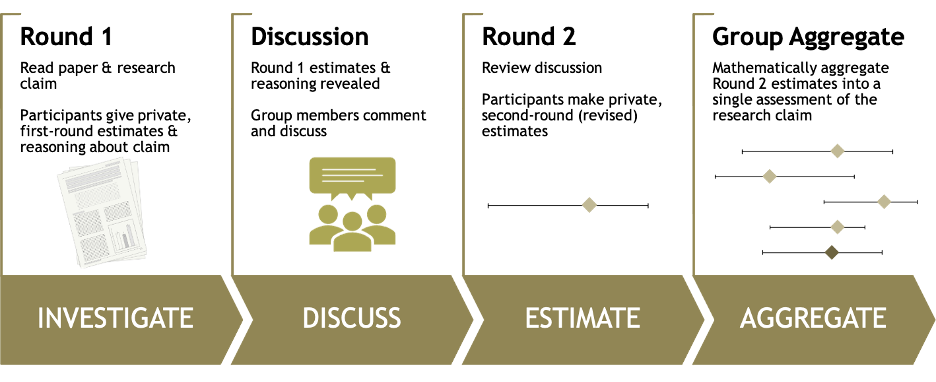
\includegraphics[keepaspectratio]{images/img_IDEA_repliCATS.png}}

}

\caption{\label{fig-1}The IDEA protocol as deployed by the repliCATS
project (reproduced with permission from Wintle et al. 2021).}

\end{figure}%

\end{tcolorbox}

\subsection{Notation and problem
formulation}\label{notation-and-problem-formulation}

First, we describe some preliminary mathematical notation used to
represent each aggregation method. The total number of forecasts
assessed, \(C\) , is indexed by \(c = 1, ..., C\). Note that in the
example dataset provided with \pkg{aggreCAT}, each forecast corresponds
to a unique research claim, indexed by \texttt{paper\_id} (see
Section~\ref{sec-package-data}). Every forecast \(c\) is assessed by
\(N\) experts is indexed by \(i = 1, ..., N\).

For each forecast, \(c\), an individual, \(i\) assesses the probability
of a some event occurring (e.g., a replication study finding a
significant result in the same direction as the original claim) by
providing up to either a single-point best estimate \(B_{i,c}\), or
three-point estimates. For three-point estimates, each expert provides
three probabilities: a lower bound \({L}_{i,c}\), an upper bound
\({U}_{i,c}\), and a best estimate \(B_{i,c}\), satisfying the
inequalities: \(0 \le L_{i,c} \le B_{i,c} \le U_{i,c} \le 1\). These
probabilities are then aggregated using one of the methods provided in
\pkg{aggreCAT} to obtain a group or aggregate probability, denoted by
\(\hat{p}_c\). The aggregated probability calculated using a specific
method is given by \(\hat{p}_{c}\left(Method \space ID \right)\). Each
aggregation is assigned a unique \(Method \space ID\) which is the
abbreviation of the mathematical operation used in calculating the
weights.

Some aggregators employ weighting schemes that are informed by proxies
for good forecasting performance whereby experts' estimates are weighted
differently by aspects, such as; engagement, openness to changing their
mind in light of new facts, extremity or informativeness of estimates,
and by statistical knowledge as measured in a quiz.

Equation~\ref{eq-weight} defines standardised notation for describing
weighted linear combinations of individual judgements where normalised
weights are denoted by \(\tilde{w} \_ method\):

\begin{equation}\protect\phantomsection\label{eq-weight}{
\hat{p}_c\left(Method \space ID \right) = \frac{1}{N}\sum_{i=1}^N \tilde{w}\_{method}_{i,c}  B_{i,c}
}\end{equation}

The suite of aggregators include methods that weight judgements at the
judgement-level, and methods that weight judgements at the
participant-level. Judgement-level weights are calculated per
participant per forecast, and therefore vary across forecasts for the
same individual. Participant-level weights are calculated per
participant, and therefore are identical across forecasts for the same
participant. We provide the option for user-supplied weights at both
levels. Some aggregation methods in \pkg{aggreCAT} rescale
judgement-level weights by some participant-level measure across all
forecasts, in which case a secondary index \(d = 1, ..., D\) is used to
denote the different forecasts that an individual has provided
judgements for, where \(D\) is the total number of forecasts that an
individual has provided judgements for.

For ease of debugging and applications across different aggregators, we
make use of \texttt{weight\_*} functions to calculate weights for
methods that require weighting. These functions are called internally
within the wrapper functions when needed, see
Table~\ref{tbl-method-summary-table} for details.

The performance of each method is evaluated by comparing the aggregated
confidence scores \(\hat{p}_c\) to the known outcomes \(j\) using
scoring rules, see Section~\ref{sec-evaluation}. For each forecast
\(c\), with known outcome, \(j\), \(j = 1\) if the event occurred and
\(j = 0\) if the event did not occur. Future work will include methods
for evaluating performance when known outcomes are non-binary, e.g.~RMSE
for counts.

\subsection{Aggregation wrapper
functions}\label{aggregation-wrapper-functions}

\pkg{aggreCAT} provides 29 aggregation methods in total, and these are
grouped by type into eight wrapper functions. These functions, denoted
by the \texttt{*WAgg} suffix (weighted aggregation), are:
\texttt{AverageWAgg()} (calculations using measures of the average),
\texttt{LinearWAgg()} (linear-weighted aggregation),
\texttt{IntervalWAgg()} (weights calculated from uncertainty bounds),
\texttt{ShiftingWAgg()} (weights calculated from estimate shifts between
rounds), \texttt{DistributionWAgg()} (averaged probability distributions
constructed from three-point elicitation), \texttt{ExtremisationWAgg()}
(applies extremisation techniques to averaged estimates),
\texttt{ReasoningWAgg()} (weights calculated from breadth of reasoning),
and \texttt{BayesianWAgg()} (Bayesian aggregation methods). The specific
aggregation \emph{method} is within each wrapper function and is applied
according to the \texttt{type} argument.

\subsubsection{`Tidy' aggregation and required
inputs}\label{sec-tidy-aggregation}

The design philosophy of \pkg{aggreCAT} is principled on `tidy' data
(Wickham 2014). Each aggregation method expects a \class{data.frame} or
\class{tibble} of judgements as its input, and returns a \class{tibble}
containing the variables \texttt{method}, \texttt{paper\_id},
\texttt{cs} and \texttt{n\_experts} (see Section~\ref{sec-AverageWAgg}
for illustration of outputs); where \texttt{method} is a character
vector corresponding to the aggregation method name specified in the
\texttt{type} argument. Each aggregation is applied as a summary
function (Wickham and Grolemund 2017), and therefore returns a single
row with a single confidence score \texttt{cs} for each claim or
\texttt{paper\_id}. The number of expert judgements summarised in the
aggregated confidence score is returned in \texttt{n\_experts}. Because
of the tidy nature of the aggregation outputs, multiple aggregation
methods can be applied to the same data with the results of all
aggregation methods row-bound together in a single \texttt{tibble} (see
the example repliCATS workflow in Section~\ref{sec-workflow}).

\subsubsection{Package data}\label{sec-package-data}

The \pkg{aggreCAT} package includes data collected by the repliCATS
project during a pilot study at a two-day workshop in the Netherlands in
July 2019, at which 25 participants assessed the replicability of 25
unique social and behavioural science research claims with known
outcomes using the IDEA protocol (Wintle et al. 2023).

The dataset is distributed over eight data objects, each containing
different types of data collected during the repliCATS project. The core
data object \texttt{data\_ratings} is a tidy \class{data.frame} of
probabilistic three-point judgements (lower bound, best estimate, upper
bound - as percentages) elicited from participants for each claim,
across two rounds of elicitation. Additional data objects capture
participants' written justifications (\texttt{data\_justifications}),
peer comments and ratings (\texttt{data\_comments}), and three
supplementary datasets collected externally to the IDEA protocol: a
statistical knowledge quiz (\texttt{data\_supp\_quiz}), qualitatively
coded reasoning categories (\texttt{data\_supp\_reasons}), and
model-derived Bayesian priors (\texttt{data\_supp\_priors}).

Known replication outcomes sourced from previous large-scale replication
projects ({Klein et al.} 2014, 2018; {Ebersole et al.} 2016; Camerer et
al. 2018; Open Science Collaboration 2015) are provided in
\texttt{data\_outcomes}. And confidence scores calculated from 22
aggregation methods on the repliCATS dataset are provided in
\texttt{data\_confidence\_scores}.

Full descriptions of each data object, are provided in the
\pkg{aggreCAT} package documentation (\texttt{?data\_ratings}) and in
the `Package Datasets' vignette available on the \pkg{aggreCAT} pkgdown
website. For further details about the dataset, see Wintle et al.
(2023).

Different aggregators require different minimum data inputs, including
the type of judgements elicited (single- or three-point estimates), the
number of elicitation rounds (one or two rounds), whether additional
data is used to construct weights. For a full summary of each
aggregation method, its \texttt{*WAgg} wrapper function and data
requirements, see Table~\ref{tbl-method-summary-table}.

\section{\texorpdfstring{Demonstrating mathematical aggregation with
\pkg{aggreCAT}}{Demonstrating mathematical aggregation with }}\label{sec-examples}

Here, we demonstrate the application of several aggregation methods in
\pkg{aggreCAT} to a subset of the repliCATS dataset. We first describe
the general workflow for applying aggregation methods in \pkg{aggreCAT}
(Box \hyperref[aggWorkflow]{2}), then demonstrate the application of
several different aggregators to a single claim with judgements from
five participants, highlighting the different data requirements and
mechanics of each method, including; the type of judgements elicited
(single- or three-point estimates), number of elicitation rounds (one or
two rounds), whether judgements are weighted at the judgement- or
participant- level, the type of mathematical operation used to combine
judgements, and whether weights are calculated internally or require
user-supplied data.

Here we demonstrate the application of aggregation methods for each
group of methods using a set of `focal claims' selected from the pilot
study dataset supplied with the \pkg{aggreCAT} package.

\begin{tcolorbox}[enhanced jigsaw, arc=.35mm, bottomrule=.15mm, breakable, colback=white, colframe=quarto-callout-color-frame, left=2mm, leftrule=.75mm, opacityback=0, rightrule=.15mm, toprule=.15mm]

\protect\phantomsection\label{aggWorkflow}
\section*{Box 2: Aggregation Workflow}\label{box-2-aggregation-workflow}
\addcontentsline{toc}{section}{Box 2: Aggregation Workflow}

All \pkg{aggreCAT} aggregation wrappers share five core arguments:
\texttt{expert\_judgements} (a tidy \class{data.frame} of expert
judgements), \texttt{type} (the aggregation method applied to
\texttt{expert\_judgements}), optional \texttt{name} (to override the
default method label), \texttt{percent\_toggle} (convert percentage
inputs to probabilities), and \texttt{round\_2\_filter} (filter to round
2 estimates).

Some methods require additional data. For example,
\texttt{ReasoningWAgg()} requires \texttt{reasons} (qualitatively coded
reasoning categories), and \texttt{BayesianWAgg()} requires
\texttt{priors} (claim-level prior information).

Each wrapper follows the same pipeline: pre-process judgements, compute
weights when needed, aggregate, then post-process results into tidy
output. Pre-processing with \texttt{pre\_process\_judgements()}
standardises inputs and filters to required rounds, elements, and
questions. For example, methods requiring only \texttt{round\ 2}
estimates remove other rounds; methods requiring only best estimates
retain only that element. Unless overridden by method-specific
requirements or users, by default, single-round methods use
\texttt{round\ 2}, single-point estimates use
\texttt{three\_point\_best}, and three-point methods use
\texttt{three\_point\_lower}, \texttt{three\_point\_upper} and
\texttt{three\_point\_best}.

When weighting is required, un-normalised weights are computed either by
dedicated helper functions or directly in the wrapper function for
simpler methods (see Table~\ref{tbl-method-summary-table}). For
instance, \texttt{ReasoningWAgg(type\ =\ "ReasonWAgg")} uses
\texttt{weight\_reason()}. Weights are then normalised within claim by
dividing each expert's weight by the claim-level weight sum.

Finally, \texttt{post\_process\_results()} returns one row per claim
with method name, confidence score, and number of aggregated experts.

\end{tcolorbox}

\subsection{Prepare focal claim data}\label{sec-focal-claims}

Below we subset the dataset \texttt{data\_ratings} to include a sample
of four focal claims with judgements from five randomly-sampled
participants. We select a single focal claim,
\texttt{paper\_id\ ==\ "108"}, to demonstrate the application of
different aggregation methods, and their unique data requirements
(Table~\ref{tbl-focal-claim}).

\begin{Shaded}
\begin{Highlighting}[]
\NormalTok{R}\SpecialCharTok{\textgreater{}} \FunctionTok{set.seed}\NormalTok{(}\DecValTok{1234}\NormalTok{)}
\NormalTok{R}\SpecialCharTok{\textgreater{}}\NormalTok{ focal\_claims }\OtherTok{\textless{}{-}}\NormalTok{ data\_ratings }\SpecialCharTok{|\textgreater{}}
\SpecialCharTok{+}\NormalTok{    dplyr}\SpecialCharTok{::}\FunctionTok{filter}\NormalTok{(paper\_id }\SpecialCharTok{\%in\%} \FunctionTok{c}\NormalTok{(}\StringTok{"24"}\NormalTok{, }\StringTok{"138"}\NormalTok{, }\StringTok{"186"}\NormalTok{, }\StringTok{"108"}\NormalTok{))}
\NormalTok{R}\SpecialCharTok{\textgreater{}} \CommentTok{\# select 5 users to highlight in focal claim demonstration}
\NormalTok{R}\SpecialCharTok{\textgreater{}}\NormalTok{ focal\_users }\OtherTok{\textless{}{-}}\NormalTok{ focal\_claims }\SpecialCharTok{|\textgreater{}}
\SpecialCharTok{+}\NormalTok{    dplyr}\SpecialCharTok{::}\FunctionTok{distinct}\NormalTok{(user\_name) }\SpecialCharTok{|\textgreater{}}
\SpecialCharTok{+}\NormalTok{    dplyr}\SpecialCharTok{::}\FunctionTok{slice\_sample}\NormalTok{(}\AttributeTok{n =} \DecValTok{5}\NormalTok{)}
\NormalTok{R}\SpecialCharTok{\textgreater{}} \CommentTok{\# filter out non{-}focal users from focal claims}
\NormalTok{R}\SpecialCharTok{\textgreater{}}\NormalTok{ focal\_claims }\OtherTok{\textless{}{-}}\NormalTok{ focal\_claims }\SpecialCharTok{|\textgreater{}}
\SpecialCharTok{+}\NormalTok{    dplyr}\SpecialCharTok{::}\FunctionTok{right\_join}\NormalTok{(focal\_users, }\AttributeTok{by =} \StringTok{"user\_name"}\NormalTok{) }\SpecialCharTok{|\textgreater{}}
\SpecialCharTok{+}\NormalTok{    dplyr}\SpecialCharTok{::}\FunctionTok{filter}\NormalTok{(stringr}\SpecialCharTok{::}\FunctionTok{str\_detect}\NormalTok{(element, }\StringTok{"three\_point"}\NormalTok{)) }\SpecialCharTok{|\textgreater{}}
\SpecialCharTok{+}\NormalTok{    dplyr}\SpecialCharTok{::}\FunctionTok{select}\NormalTok{(}\SpecialCharTok{{-}}\NormalTok{question)}
\NormalTok{R}\SpecialCharTok{\textgreater{}}\NormalTok{ focal\_claim\_108 }\OtherTok{\textless{}{-}}\NormalTok{ focal\_claims }\SpecialCharTok{|\textgreater{}}
\SpecialCharTok{+}\NormalTok{    dplyr}\SpecialCharTok{::}\FunctionTok{filter}\NormalTok{(paper\_id }\SpecialCharTok{==} \StringTok{"108"}\NormalTok{)}
\NormalTok{R}\SpecialCharTok{\textgreater{}}\NormalTok{ focal\_claims}
\end{Highlighting}
\end{Shaded}

\begin{verbatim}
# A tibble: 120 x 6
   round   paper_id user_name  element           value group
   <chr>   <chr>    <chr>      <chr>             <dbl> <chr>
 1 round_1 108      lvr6dwbqag three_point_upper    90 UOM1 
 2 round_1 108      lvr6dwbqag three_point_lower    40 UOM1 
 3 round_1 108      lvr6dwbqag three_point_best     65 UOM1 
 4 round_1 108      f35wd3nhdz three_point_upper    60 UOM3 
 5 round_1 108      f35wd3nhdz three_point_lower    40 UOM3 
 6 round_1 108      f35wd3nhdz three_point_best     51 UOM3 
 7 round_1 108      kf7fxabzu0 three_point_lower    70 UOM3 
 8 round_1 108      kf7fxabzu0 three_point_upper    90 UOM3 
 9 round_1 108      kf7fxabzu0 three_point_best     80 UOM3 
10 round_1 108      g31jx5dffs three_point_lower    70 UOM4 
# i 110 more rows
\end{verbatim}

\begin{table}[H]

\caption{\label{tbl-focal-claim}Example of expert judgement data for a
single claim.}

\centering{

\centering
\begin{tblr}[         %% tabularray outer open
]                     %% tabularray outer close
{                     %% tabularray inner open
colspec={Q[]Q[]Q[]Q[]Q[]},
hline{2}={1-5}{solid, black, 0.05em},
hline{1}={1-5}{solid, black, 0.08em},
hline{7}={1-5}{solid, black, 0.08em},
}                     %% tabularray inner close
Claim ID & Participant & Lower Bound & Best Estimate & Upper Bound \\
108 & g31jx5dffs & 70 & 85 & 90 \\
108 & 5nuvx01cj5 & 70 & 80 & 90 \\
108 & f35wd3nhdz & 60 & 80 & 90 \\
108 & lvr6dwbqag & 40 & 65 & 90 \\
108 & kf7fxabzu0 & 50 & 60 & 70 \\
\end{tblr}

}

\end{table}%

\subsection{Unweighted linear combination of
judgements}\label{sec-AverageWAgg}

We first demonstrate the mechanics of mathematical aggregation and its
implementation using the \pkg{aggreCAT} package with the simplest,
unweighted aggregation wrapper, \texttt{AverageWAgg()}.

The \fct{AverageWAgg} wrapper function implements several methods that
calculate different types of unweighted averaged best-estimates (see
\texttt{?AverageWAgg}). The output is a \class{tibble} containing the
method name, paper ID, confidence score, and number of experts whose
judgements were aggregated. All other aggregation methods take this
underlying computational blueprint, and expand on it according to the
aggregation methods' requirements (See Box \hyperref[aggWorkflow]{2} for
details).

Below we illustrate the mechanics of the arithmetic mean method
`\texttt{ArMean}', which takes the unweighted linear average of the best
estimates, \(B_{i,c}\), across all \(N\) experts for a given claim \(c\)
to calculate the aggregated confidence score \(\hat{p}_c\)
(Equation~\ref{eq-ArMean}). The \texttt{type} argument is used across
all aggregation wrapper functions to specify the method of aggregation.
Below we apply \texttt{ArMean} to the focal claim \texttt{108}
(Table~\ref{tbl-focal-claim}), which has judgements from five
participants. Note that the \texttt{AverageWAgg()} wrapper function
implements several methods that calculate different types of unweighted
averaged best-estimates (see \texttt{?AverageWAgg}), and in this case,
we specify \texttt{type\ =\ "ArMean"} to apply the \texttt{ArMean}
method.

\begin{equation}\protect\phantomsection\label{eq-ArMean}{
\hat{p}_c\left(ArMean \right ) = \frac{1}{N}\sum_{i=1}^N B_{i,c}
}\end{equation}

\begin{Shaded}
\begin{Highlighting}[]
\NormalTok{R}\SpecialCharTok{\textgreater{}}\NormalTok{ focal\_claims }\SpecialCharTok{|\textgreater{}}
\SpecialCharTok{+}\NormalTok{    dplyr}\SpecialCharTok{::}\FunctionTok{filter}\NormalTok{(paper\_id }\SpecialCharTok{==} \StringTok{"108"}\NormalTok{) }\SpecialCharTok{|\textgreater{}}
\SpecialCharTok{+}    \FunctionTok{AverageWAgg}\NormalTok{(}\AttributeTok{type =} \StringTok{"ArMean"}\NormalTok{)}
\end{Highlighting}
\end{Shaded}

\begin{verbatim}
# A tibble: 1 x 4
  method paper_id    cs n_experts
  <chr>  <chr>    <dbl>     <int>
1 ArMean 108         74         5
\end{verbatim}

\begin{figure}[H]

\centering{

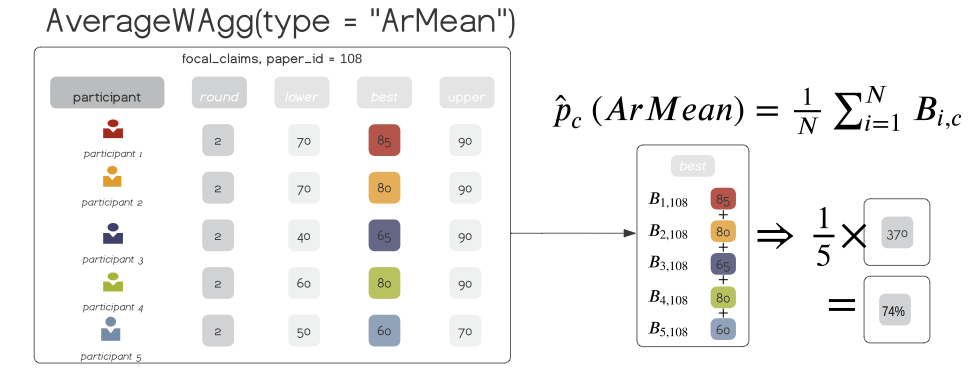
\includegraphics[width=6.25in,height=\textheight,keepaspectratio]{images/ArMean.png}

}

\caption{\label{fig-ArMean}ArMean with \texttt{AverageWAgg()} uses the
Estimates (shown in colour) from each participant to compute the mean.
We illustrate this using a single claim \texttt{108} for a subset of 5
out of 25 participants from the \texttt{data\_ratings} dataset. Note
that the data representations in this figure are for explanatory
purposes only, the data in the actual aggregation is tidy, with long
form structure and format.}

\end{figure}%

Other aggregation wrapper functions that do not weight judgements
include: \texttt{ExtremisationWAgg()} \texttt{DistributionWAgg()} (see
Table~\ref{tbl-method-summary-table}).

\subsection{Weighted linear combination of
Judgements}\label{weighted-linear-combination-of-judgements}

To improve the calibration, accuracy and informativeness of aggregated
judgements, many aggregation methods in \pkg{aggreCAT} use weighting
schemes to differentially weight individual judgements according to both
measures and proxies of forecasting performance. In the absence of
measures of experts' prior performance, proxies for forecasting
performance, such as breadth and variability of qualitative reasons used
by experts to justify their judgements (see
Section~\ref{sec-ReasonWAgg}), can be used to form weights ({Hanea et
al.} 2021).

Weights may be calculated at the judgement-level or participant-level.
Judgement-level weights are calculated per participant per claim, and
therefore vary across claims for the same participant. Participant-level
weights are calculated per participant, and therefore are identical
across claims for the same participant.

\subsubsection{Judgement-level weights}\label{sec-IntervalWAgg}

\texttt{IntervalWAgg} uses judgement-level weights by aggregating
linearly weighted best estimates with weights determined by the interval
width of the forecast. The \texttt{IntWAgg} method implemented by the
\texttt{IntervalWAgg()} function weights each participant's best
estimate \(B_{i,c}\) by the width of their uncertainty intervals,
i.e.~the difference between an individual's upper \({U}_{i,c}\) and
lower bounds \({L}_{i,c}\). The intuition behind this weighting scheme
is that participants who provide narrower uncertainty intervals are more
confident in their estimate, and therefore likely to be more accurate
for the target forecast. Hence, participants with narrower intervals are
weighted more heavily in the aggregation than those with wider
intervals.

For a given claim \(c\), a vector of weights for all individuals is
calculated from their upper and lower estimates using the weighting
function, \fct{weight_interval}, which calculates the interval width for
each individual's estimate for the target forecast
(Equation~\ref{eq-weightInterval}). The weights are then normalised
across the claim (by dividing each weight by the sum of all weights per
claim). Normalised weights are then multiplied by the corresponding
individual's best estimates \(B_{i,c}\) and summed together into a
single confidence score (Equation~\ref{eq-IntWAgg}).

\begin{equation}\protect\phantomsection\label{eq-weightInterval}{
w\_Interval_{i,c} = \frac{1}{U_{i,c} - L_{i,c}}
}\end{equation}

\begin{equation}\protect\phantomsection\label{eq-IntWAgg}{
\hat{p}_c(IntWAgg) = \sum_{i=1}^N \tilde{w}\_Interval_{i,c}B_{i,c}
}\end{equation}

\subsubsection{Judgement-level weights rescaled by participant-level
behaviour}\label{sec-IndIntWAgg}

To account for differences in interval widths across forecasts,
judgement-level weights can be rescaled. In \texttt{IndIntWAgg} each
participant's best estimate \(B_{i,c}\) is weighted by their interval
width for forecast \(c\) relative to their average interval width across
all forecasts. When the interval width for a given forecast is narrower
than the participant's average interval width across forecasts, it
implies greater confidence and potentially better forecasting
performance.

\texttt{weight\_nIndivInterval()} computes this rescaled weight
(Equation~\ref{eq-weightnIndivInterval}). The weights are then
normalised within each forecast, multiplied by \(B_{i,c}\), and summed
to give the aggregated confidence score (Equation~\ref{eq-IndIntWAgg}).

\begin{equation}\protect\phantomsection\label{eq-weightnIndivInterval}{
w\_nIndivInterval_{i,c}= \frac{1}{\frac{U_{i,c} - L_{i,c}}{max({ (U_{i,d} - L_{i,d}): d = 1,\dots, C})}}
}\end{equation}

\begin{equation}\protect\phantomsection\label{eq-IndIntWAgg}{
\hat{p}_c\left( IndIntWAgg \right) = \sum_{i=1}^N \tilde{w}\_nIndivInterval_{i,c}B_{i,c}
}\end{equation}

The \texttt{IntervalWAgg()} wrapper function implements several methods
that calculate different types of weighted linear combinations of best
estimates with weights calculated from uncertainty bounds (see
\texttt{?IntervalWAgg}). Let's apply both the \texttt{IntWAgg} and
\texttt{IndIntWAgg} methods to the focal claim \texttt{108}
(Table~\ref{tbl-focal-claim}) using \texttt{IntervalWAgg()}, by
specifying the \texttt{type} argument accordingly:

\begin{Shaded}
\begin{Highlighting}[]
\NormalTok{R}\SpecialCharTok{\textgreater{}} \FunctionTok{bind\_rows}\NormalTok{(}
\SpecialCharTok{+}\NormalTok{    focal\_claim\_108 }\SpecialCharTok{|\textgreater{}}
\SpecialCharTok{+}      \FunctionTok{IntervalWAgg}\NormalTok{(}\AttributeTok{type =} \StringTok{"IntWAgg"}\NormalTok{),}
\SpecialCharTok{+}\NormalTok{    focal\_claim\_108 }\SpecialCharTok{|\textgreater{}}
\SpecialCharTok{+}      \FunctionTok{IntervalWAgg}\NormalTok{(}\AttributeTok{type =} \StringTok{"IndIntWAgg"}\NormalTok{)}
\SpecialCharTok{+}\NormalTok{  )}
\end{Highlighting}
\end{Shaded}

\begin{verbatim}
# A tibble: 2 x 4
  method     paper_id    cs n_experts
  <chr>      <chr>    <dbl>     <int>
1 IntWAgg    108       74.8         5
2 IndIntWAgg 108       74           5
\end{verbatim}

Other wrapper functions that weight estimates at the judgement-level
include: \texttt{ShiftingWAgg()}, which weights estimates based on
shifts in expert opinions between rounds when judgements are elicited
using the IDEA protocol (or similar, Box \hyperref[ideaProtocol]{1});
\texttt{ReasoningWAgg()}, which weights estimates by the breadth of
reasoning provided in support of the estimate (see
Section~\ref{sec-ReasonWAgg}); and several methods implemented by the
\texttt{LinearWAgg()} function, including \texttt{DistLimitWAgg}, which
weights judgements based on the distance of estimates from the limits of
the interval, \texttt{GranWAgg}, which calculates weights based on the
granularity of estimates, and \texttt{OutWAgg}, which downweights
outlier estimates.

\subsubsection{Participant-level
weights}\label{participant-level-weights}

\texttt{VarIndIntWAgg} uses participant-level weights by weighting each
participant's best estimate \(B_{i,c}\) by the variability of their
interval widths across forecasts relative to other participants. This
method assumes that participants who show greater variability in their
interval widths across forecasts are more responsive to the supporting
evidence of different claims, and therefore more likely to be accurate
forecasters.

\begin{equation}\protect\phantomsection\label{eq-weightVarIndInt}{
w\_varIndivInterval_{i}= var{(U_{i,c} - L_{i,c}): c = 1,\dots, C}
}\end{equation}

Where the variance \(\texttt{var}\) is calculated across claims for each
participant, and the weights are then normalised across participants,
multiplied by \(B_{i,c}\), and summed to give the aggregated confidence
score (Equation~\ref{eq-VarIndIntWAgg}):
\begin{equation}\protect\phantomsection\label{eq-VarIndIntWAgg}{
\hat{p}_c\left( VarIndIntWAgg \right) = \sum_{i=1}^N \tilde{w}\_varIndivInterval_{i}B_{i,c}
}\end{equation}

\begin{Shaded}
\begin{Highlighting}[]
\NormalTok{R}\SpecialCharTok{\textgreater{}}\NormalTok{ focal\_claims }\SpecialCharTok{|\textgreater{}}
\SpecialCharTok{+}    \FunctionTok{IntervalWAgg}\NormalTok{(}\AttributeTok{type =} \StringTok{"VarIndIntWAgg"}\NormalTok{)}
\end{Highlighting}
\end{Shaded}

\begin{verbatim}
# A tibble: 4 x 4
  method        paper_id    cs n_experts
  <chr>         <chr>    <dbl>     <int>
1 VarIndIntWAgg 108       74.6         5
2 VarIndIntWAgg 138       68.8         5
3 VarIndIntWAgg 186       57.5         5
4 VarIndIntWAgg 24        21.1         5
\end{verbatim}

See \texttt{?IntervalWAgg} for other methods that calculate different
types of weighted linear combinations of best estimates with weights
calculated from uncertainty bounds, and
Table~\ref{tbl-method-summary-table} for a summary of all methods that
use participant-level weights.

\subsection{Weighted linear combination of judgements with user-supplied
weights}\label{weighted-linear-combination-of-judgements-with-user-supplied-weights}

\pkg{aggreCAT} provides several methods that utilise external data to
construct weights for the aggregation of expert judgements.
\texttt{LinearWAgg()} provides a flexible wrapper function for
\emph{applying} user-supplied weights to the best estimates \(B_{i,c}\)
at either the judgement-level or participant-level. While, some
aggregators utilise external data to \emph{construct} weights internally
within the wrapper functions, such as \texttt{ReasoningWAgg()} and
\texttt{BayesianWAgg()} (see Section~\ref{sec-ReasonWAgg} and
Section~\ref{sec-BayesianWAgg}).

\subsubsection{User-supplied weights}\label{sec-QuizWAgg}

Using the \texttt{LinearWAgg()} wrapper function, any user-supplied
weight can be applied at either the participant-level
(\texttt{type\ =\ "Participant"}) or the judgement-level
(\texttt{type\ =\ "Judgement"}). We show how to apply the
\texttt{QuizWAgg} method described in ({Hanea et al.} 2021) to the focal
claim with \texttt{LinearWAgg()}, which weights each participant's best
estimate \(B_{i,c}\) by their score on a on a statistical knowledge quiz
under the assumption that participants with higher statistical knowledge
are more likely to be accurate forecasters, and therefore should be
weighted more heavily in the aggregation than those with lower
statistical knowledge.

\texttt{weights} are constructed from the \texttt{data\_supp\_quiz}
dataset, which is a dataset of quiz scores for each participant in the
repliCATS pilot study (See \texttt{?data\_supp\_quiz} for details about
the dataset). The quiz dataset contains multiple score variables to
choose as weights for the \texttt{QuizWAgg} method. We rename our chosen
quiz score variable to \texttt{weight} to meet the requirements of the
\texttt{LinearWAgg()}. The weights are then normalised across
participants, multiplied by \(B_{i,c}\), and summed to give the
aggregated confidence score. To customise the name of the method
returned in our output, we set the \texttt{name} argument to
\texttt{QuizWAgg}:

\begin{Shaded}
\begin{Highlighting}[]
\NormalTok{focal\_claim\_108 }\SpecialCharTok{|\textgreater{}}
  \FunctionTok{LinearWAgg}\NormalTok{(}
    \AttributeTok{type =} \StringTok{"Participant"}\NormalTok{,}
    \AttributeTok{weights =}\NormalTok{ data\_supp\_quiz }\SpecialCharTok{|\textgreater{}}
      \FunctionTok{rename}\NormalTok{(}\AttributeTok{weight =}\NormalTok{ quiz\_score),}
    \AttributeTok{name =} \StringTok{"QuizWAgg"}
\NormalTok{  )}
\end{Highlighting}
\end{Shaded}

\begin{verbatim}
# A tibble: 1 x 4
  method   paper_id    cs n_experts
  <chr>    <chr>    <dbl>     <int>
1 QuizWAgg 108       73.4         5
\end{verbatim}

In this way users can specify their own custom weights in addition to
those described by {Hanea et al.} (2021) by preparing a dataset of
weights and parsing this to \texttt{LinearWAgg()}'s \texttt{weights}
argument. The dataset of weights must contain a column named
\texttt{weight} containing the weight values, and a column that can be
used to join the weights to the \texttt{expert\_judgements} dataset by
participant (e.g.~\texttt{user\_name}) or by judgement
(e.g.~\texttt{paper\_id} and \texttt{user\_name}).

\subsubsection{\texorpdfstring{Reasoning-based weights
\texttt{ReasonWAgg()}}{Reasoning-based weights ReasonWAgg()}}\label{sec-ReasonWAgg}

The \texttt{ReasoningWAgg()} function, which implements the
\texttt{ReasonWAgg} method, requires a dataset of qualitatively coded
reasons that experts provided to justify their numeric estimates.
\texttt{ReasonWAgg} weights each participant's best estimate \(B_{i,c}\)
by the number of unique reasoning categories they used to justify their
estimates for the target forecast \(c\), assuming that participants who
use a greater breadth of reasoning categories to justify their estimates
are more likely to be accurate forecasters.

The weighting function \texttt{weight\_reason()} counts the number of
unique reasons used by each participant for each claim, and uses this as
a proxy for forecasting performance (Equation~\ref{eq-weightReason}).
Here, \(r = 1, \dots, R\) indexes the distinct reason categories
available in the coded dataset, and \(R\) is the total number of unique
reason categories that any participant could use in justifying their
estimates. The more unique a participant uses to justify their
estimates, the higher their weight in the aggregation. The weights are
then normalised across the claim and multiplied by the corresponding
individual's best estimates \(B_{i,c}\) and summed together into a
single confidence score (Equation~\ref{eq-ReasonWAgg}).

\begin{equation}\protect\phantomsection\label{eq-weightReason}{
w\_reason_{i,c}= \sum_{r=1}^R I\left(\text{reason}_{i,c} = r\right)
}\end{equation}

\begin{equation}\protect\phantomsection\label{eq-ReasonWAgg}{
\hat{p}_c\left(\texttt{ReasonWAgg} \right ) = \frac{1}{N}\sum_{i=1}^N \tilde{w}\_{reason}_{i,c}  B_{i,c}
}\end{equation}

Below we apply the \texttt{ReasonWAgg} method to the focal claim
\texttt{108} using the \fct{ReasoningWAgg} wrapper function. First, we
prepare the dataset of reasons by filtering \texttt{data\_supp\_reasons}
to include only the focal users who assessed claim \texttt{108}.

We reshape the output to illustrate the number of unique reasoning
categories used by each participant to justify their estimates for claim
\texttt{108} (Table~\ref{tbl-focal-claim-reasons}). Each column
corresponds to a unique reason category, and the value in each cell
indicates whether a participant used that reason category (1) or not (0)
to justify their estimates for claim \texttt{108}. The total number of
unique reasons used by each participant is then calculated by summing
across the reason category columns.

\begin{table}

\caption{\label{tbl-focal-claim-reasons}Reasoning data for focal claim
\texttt{108} for a sample of reasoning categories. The dataset of
reasons is used to construct weights for the \texttt{ReasonWAgg} method,
which weights each participant's best estimate by the number of unique
reasoning categories they used to justify their estimates for the target
forecast (see \texttt{?data\_supp\_reasons} for details). Each column
corresponds to a unique reason category, and the value in each cell
indicates whether a participant used that reason category (1) or not
(0). The total number of unique reasons used by each participant is
calculated by summing across the reason category columns.}

\centering{

\centering
\begin{tblr}[         %% tabularray outer open
]                     %% tabularray outer close
{                     %% tabularray inner open
width={1\linewidth},
colspec={X[0.16]X[0.21]X[0.21]X[0.21]X[0.21]},
hline{2}={1-5}{solid, black, 0.05em},
hline{1}={1-5}{solid, black, 0.08em},
hline{7}={1-5}{solid, black, 0.08em},
}                     %% tabularray inner close
Participant & Plausibility & Population or subject characteristics (sampling practices) & Revision statements & Significance statistical (p-value etc ) \\
5nuvx01cj5 & 1 & 0 & 1 & 1 \\
f35wd3nhdz & 1 & 0 & 0 & 0 \\
g31jx5dffs & 1 & 0 & 0 & 0 \\
kf7fxabzu0 & 1 & 0 & 0 & 0 \\
lvr6dwbqag & 1 & 1 & 0 & 0 \\
\end{tblr}

}

\end{table}%

Then we apply the \texttt{ReasonWAgg} method to compute a confidence
score for claim \texttt{108} weighting participants' best estimates by
the number of unique reasoning categories they used to justify their
estimates for that claim.

\begin{Shaded}
\begin{Highlighting}[]
\NormalTok{R}\SpecialCharTok{\textgreater{}}\NormalTok{ focal\_claims }\SpecialCharTok{|\textgreater{}}
\SpecialCharTok{+}\NormalTok{    dplyr}\SpecialCharTok{::}\FunctionTok{filter}\NormalTok{(paper\_id }\SpecialCharTok{==} \StringTok{"108"}\NormalTok{) }\SpecialCharTok{|\textgreater{}}
\SpecialCharTok{+}    \FunctionTok{ReasoningWAgg}\NormalTok{(}\AttributeTok{type =} \StringTok{"ReasonWAgg"}\NormalTok{, }\AttributeTok{reasons =}\NormalTok{ data\_supp\_reasons)}
\end{Highlighting}
\end{Shaded}

\begin{verbatim}
# A tibble: 1 x 4
  method     paper_id    cs n_experts
  <chr>      <chr>    <dbl>     <int>
1 ReasonWAgg 108       74.4         5
\end{verbatim}

\blandscape

\begin{figure}[!t]

\centering{

\includegraphics[width=9.68in,height=\textheight,keepaspectratio]{aggreCAT_2_files/figure-pdf/fig-ReasonWAgg-1.png}

}

\caption{\label{fig-ReasonWAgg}Illustration of the \texttt{ReasonWAgg}
aggregation method for a subset of five participants who assessed claim
\texttt{108}. \texttt{ReasonWAgg} is applied using the wrapper function
\texttt{ReasoningWAgg()} and exemplifies aggregation methods that use
supplementary data (\texttt{data\_supp\_ReasonWAgg}) collected
externally to the IDEA protocol in the construction of weights and
subsequent calculation of confidence scores. Weights are constructed by
taking the sum of the number of unique reasons made in support of
quantitative estimates for each participant, for the target forecast.}

\end{figure}%

\elandscape

\subsection{Bayesian aggregation methods}\label{sec-BayesianWAgg}

While most aggregation methods in \pkg{aggreCAT} are weighted linear
combinations of best estimates, the \texttt{BayesianWAgg()} aggregation
family takes a model-based approach to computing confidence scores. It
implements two variants that use elicited best estimates as data with
which to update prior distributions of forecasts: \texttt{BayTriVar} and
\texttt{BayPriorsAgg}. Both methods use the same underlying Bayesian
model, but differ in how the prior distributions are specified. The
\texttt{BayTriVar} method assumes forecast-specific prior means, while
\texttt{BayPriorsAgg} allows users to specify their own priors.

The model in \texttt{BayesianWAgg} incorporates uncertainty from three
sources: (i) \emph{judgement-level variability}, based on the width of
each participant's uncertainty interval for the target forecast; (ii)
\emph{participant-level variability}, defined as variation in each
participant's best estimates across all forecasts they assessed; and
(iii) \emph{forecast-level variability}, defined as variation in best
estimates across all participants for a given forecast. The confidence
score is then taken as the median of the posterior distribution.

Below we apply the Bayesian Triple Variability method \texttt{BayTriVar}
to the focal claim, which expects best estimates in the form of
probabilities. We toggle the argument \texttt{percent\_toggle} to
\texttt{TRUE} to convert percentage inputs to probabilities in the data
parsed to the \texttt{expert\_judgement} argument. Although we compute
the confidence score for a single claim only, the model computes
participant-level weights using data from all forecasts within
\texttt{expert\_judgements}. Consequently we filter the aggregated
confidence scores for claim \texttt{108} \emph{after} applying the
aggregation method to the full dataset of claims:

\begin{Shaded}
\begin{Highlighting}[]
\NormalTok{R}\SpecialCharTok{\textgreater{}}\NormalTok{ focal\_claims }\SpecialCharTok{|\textgreater{}}
\SpecialCharTok{+}    \FunctionTok{BayesianWAgg}\NormalTok{(}\AttributeTok{type =} \StringTok{"BayTriVar"}\NormalTok{, }\AttributeTok{percent\_toggle =} \ConstantTok{TRUE}\NormalTok{) }\SpecialCharTok{|\textgreater{}}
\SpecialCharTok{+}\NormalTok{    dplyr}\SpecialCharTok{::}\FunctionTok{filter}\NormalTok{(paper\_id }\SpecialCharTok{==} \StringTok{"108"}\NormalTok{)}
\end{Highlighting}
\end{Shaded}

\begin{verbatim}
# A tibble: 1 x 4
  method    paper_id    cs n_experts
  <chr>     <chr>    <dbl>     <int>
1 BayTriVar 108      0.699         5
\end{verbatim}

Because \texttt{BayesianWAgg()} computes participant-level weights using
data from all forecasts, the aggregated estimates are sensitive to the
input data. This is also true for any aggregators that re-scale
judgement-level weights with participant-level values, such as
\texttt{IndIntWAgg} (see Section~\ref{sec-IntervalWAgg}). As such, when
calculating the confidence score for a single forecast, the user should
ensure that the all available forecasts are parsed to
\texttt{expert\_judgements} before applying the aggregation method, and
then filter the aggregated estimates for the target forecast after
aggregation.

Below we illustrate this point by calculating the confidence score for
claim \texttt{108} using \texttt{BayTriVar} with a different input
dataset, \texttt{data\_ratings}, which contains judgements for all
claims in the repliCATS pilot study. We apply \texttt{BayTriVar} to the
full dataset of claims, and then filter the aggregated confidence scores
for claim \texttt{108} \emph{after} applying the aggregation method to
the full dataset of claims:

\begin{Shaded}
\begin{Highlighting}[]
\NormalTok{data\_ratings }\SpecialCharTok{|\textgreater{}}
  \FunctionTok{BayesianWAgg}\NormalTok{(}\AttributeTok{type =} \StringTok{"BayTriVar"}\NormalTok{, }\AttributeTok{percent\_toggle =} \ConstantTok{TRUE}\NormalTok{) }\SpecialCharTok{|\textgreater{}}
\NormalTok{  dplyr}\SpecialCharTok{::}\FunctionTok{filter}\NormalTok{(paper\_id }\SpecialCharTok{==} \StringTok{"108"}\NormalTok{)}
\end{Highlighting}
\end{Shaded}

\begin{verbatim}
# A tibble: 1 x 4
  method    paper_id    cs n_experts
  <chr>     <chr>    <dbl>     <int>
1 BayTriVar 108      0.748        25
\end{verbatim}

Notice that the confidence score for claim \texttt{108} differs between
the two applications of \texttt{BayTriVar}, depending on which input
data was used to compute participant-level weights. This illustrates the
importance of ensuring that all available forecasts are parsed to
\texttt{expert\_judgements} when applying aggregation methods that use
participant-level weights, and then filtering the aggregated estimates
for the target forecast after aggregation.

\section{An illustrative workflow for use in real study
contexts}\label{sec-workflow}

Throughout the SCORE program, 752 participants assessed more than 4000
unique claims using the repliCATS IDEA protocol, between 7th July 2019
and 25 November 2021 (Mody et al. 2026). This required batch aggregation
over multiple claims, and to generate confidence scores for multiple
claims. We also applied multiple aggregation methods to the same claim
so that we could compare and evaluate the different aggregation methods.
We expect that these are not uncommon use-cases, therefore we now
demonstrate a general workflow for using the \pkg{aggreCAT} package to
aggregate expert judgements using pilot data from DARPA SCORE program
generated by the repliCATS project.

\subsection{Generating multiple
forecasts}\label{generating-multiple-forecasts}

The modular and tidy design of the aggregation functions in
\pkg{aggreCAT} (see Box \hyperref[aggWorkflow]{2} and
Section~\ref{sec-tidy-aggregation}) supports batch aggregation of
judgements across multiple forecasts using multiple methods so that the
user is free to focus their attention on the interpretation and analysis
of the forecasts, rather than on data processing and implementation of
the aggregation methods. Below we apply the \texttt{ArMean} aggregation
method to 25 claims evaluated by 25 participants simultaneously:

\begin{Shaded}
\begin{Highlighting}[]
\FunctionTok{AverageWAgg}\NormalTok{(data\_ratings, }\AttributeTok{type =} \StringTok{"ArMean"}\NormalTok{)}
\end{Highlighting}
\end{Shaded}

\begin{verbatim}
# A tibble: 25 x 4
   method paper_id    cs n_experts
   <chr>  <chr>    <dbl>     <int>
 1 ArMean 100       70.6        25
 2 ArMean 102       30.8        25
 3 ArMean 103       62.5        25
 4 ArMean 104       47.1        25
 5 ArMean 106       36.5        25
 6 ArMean 108       71.8        25
 7 ArMean 109       72.5        25
 8 ArMean 116       62.6        25
 9 ArMean 118       54.8        25
10 ArMean 133       59.9        25
# i 15 more rows
\end{verbatim}

\subsection{Comparing and evaluating aggregation
methods}\label{sec-evaluation}

In real study contexts, such as that of the repliCATS project, it is of
interest to compute confidence scores using multiple aggregation methods
so that their performance might be evaluated and compared. Since
different methods offer different mathematical properties, and therefore
might be more or less appropriate depending on the purpose of the
aggregation and forecasting, a researcher or analyst might want to check
how the different assumptions embedded in different aggregation methods
influence the final confidence scores for a forecast -- i.e.~how robust
are the results to different methods and therefore to different
assumptions?

From a computational perspective, multiple aggregation methods must
first be applied to the forecast prior to comparison and evaluation.
This can be achieved by applying each different aggregation method to
\texttt{focal\_claims}, and binding the results together with
\pkg{dplyr}'s \fct{bind_rows}. However, more elegant and succinct
solutions can be implemented using \pkg{purrr}'s \fct{map_dfr} function
(Henry and Wickham (2020), see
Listing~\ref{lst-multi-method-workflow-non-supp} and
Listing~\ref{lst-multi-method-workflow-both}).

\begin{Shaded}
\begin{Highlighting}[]
\NormalTok{R}\SpecialCharTok{\textgreater{}}\NormalTok{ confidenceSCOREs }\OtherTok{\textless{}{-}}
\SpecialCharTok{+}\NormalTok{    dplyr}\SpecialCharTok{::}\FunctionTok{bind\_rows}\NormalTok{(}
\SpecialCharTok{+}      \FunctionTok{AverageWAgg}\NormalTok{(data\_ratings,}
\SpecialCharTok{+}        \StringTok{"ArMean"}\NormalTok{,}
\SpecialCharTok{+}        \AttributeTok{percent\_toggle =} \ConstantTok{TRUE}
\SpecialCharTok{+}\NormalTok{      ),}
\SpecialCharTok{+}      \FunctionTok{IntervalWAgg}\NormalTok{(data\_ratings,}
\SpecialCharTok{+}        \StringTok{"IndIntWAgg"}\NormalTok{,}
\SpecialCharTok{+}        \AttributeTok{percent\_toggle =} \ConstantTok{TRUE}
\SpecialCharTok{+}\NormalTok{      ),}
\SpecialCharTok{+}      \FunctionTok{IntervalWAgg}\NormalTok{(data\_ratings,}
\SpecialCharTok{+}        \StringTok{"IntWAgg"}\NormalTok{,}
\SpecialCharTok{+}        \AttributeTok{percent\_toggle =} \ConstantTok{TRUE}
\SpecialCharTok{+}\NormalTok{      ),}
\SpecialCharTok{+}      \FunctionTok{ShiftingWAgg}\NormalTok{(data\_ratings,}
\SpecialCharTok{+}        \StringTok{"ShiftWAgg"}\NormalTok{,}
\SpecialCharTok{+}        \AttributeTok{percent\_toggle =} \ConstantTok{TRUE}
\SpecialCharTok{+}\NormalTok{      ),}
\SpecialCharTok{+}      \FunctionTok{BayesianWAgg}\NormalTok{(data\_ratings,}
\SpecialCharTok{+}        \StringTok{"BayTriVar"}\NormalTok{,}
\SpecialCharTok{+}        \AttributeTok{percent\_toggle =} \ConstantTok{TRUE}
\SpecialCharTok{+}\NormalTok{      ),}
\SpecialCharTok{+}      \FunctionTok{ReasoningWAgg}\NormalTok{(data\_ratings,}
\SpecialCharTok{+}        \AttributeTok{reasons =}\NormalTok{ data\_supp\_reasons,}
\SpecialCharTok{+}        \AttributeTok{percent\_toggle =} \ConstantTok{TRUE}
\SpecialCharTok{+}\NormalTok{      )}
\SpecialCharTok{+}\NormalTok{    )}
\NormalTok{R}\SpecialCharTok{\textgreater{}}\NormalTok{ confidenceSCOREs}
\end{Highlighting}
\end{Shaded}

\begin{verbatim}
# A tibble: 150 x 4
   method paper_id    cs n_experts
   <chr>  <chr>    <dbl>     <int>
 1 ArMean 100      0.706        25
 2 ArMean 102      0.308        25
 3 ArMean 103      0.625        25
 4 ArMean 104      0.471        25
 5 ArMean 106      0.365        25
 6 ArMean 108      0.718        25
 7 ArMean 109      0.725        25
 8 ArMean 116      0.626        25
 9 ArMean 118      0.548        25
10 ArMean 133      0.599        25
# i 140 more rows
\end{verbatim}

After generating confidence scores using various aggregation methods, we
then evaluate the forecasts. We evaluated the repliCATS pilot study
forecasts against the outcomes of previous, high-powered replication
studies ({Hanea et al.} 2021), which are contained in the
\texttt{data\_outcomes} dataset published with \pkg{aggreCAT}.
\texttt{data\_outcomes} records the binary replication outcome
(\texttt{outcome}: \texttt{1} if the claim successfully replicated,
\texttt{0} if not) for each \texttt{paper\_id}, sourced from previous
large-scale replication projects ({Klein et al.} 2014, 2018; {Ebersole
et al.} 2016; Camerer et al. 2018; Open Science Collaboration 2015):

\begin{Shaded}
\begin{Highlighting}[]
\NormalTok{R}\SpecialCharTok{\textgreater{}}\NormalTok{ data\_outcomes }\SpecialCharTok{|\textgreater{}}
\SpecialCharTok{+}    \FunctionTok{head}\NormalTok{()}
\end{Highlighting}
\end{Shaded}

\begin{verbatim}
# A tibble: 6 x 2
  paper_id outcome
  <chr>      <dbl>
1 100            1
2 102            0
3 103            0
4 104            1
5 106            0
6 108            1
\end{verbatim}

The function \fct{confidence_score_evaluation} evaluates a set of
aggregated forecasts or confidence scores against a set of known or
observed outcomes, returning the Area Under the ROC Curve (AUC), the
Brier score, and classification accuracy and correlation of each method
(Table~\ref{tbl-multi-method-workflow-eval}):

\begin{Shaded}
\begin{Highlighting}[]
\NormalTok{R}\SpecialCharTok{\textgreater{}} \FunctionTok{confidence\_score\_evaluation}\NormalTok{(}
\SpecialCharTok{+}\NormalTok{    confidenceSCOREs,}
\SpecialCharTok{+}\NormalTok{    data\_outcomes}
\SpecialCharTok{+}\NormalTok{  )}
\end{Highlighting}
\end{Shaded}

\begin{table}[H]

\caption{\label{tbl-multi-method-workflow-eval}AUC and Classification
Accuracy for forecasts from the aggregation methods \texttt{ShiftWAgg},
\texttt{ArMean}, \texttt{IntWAgg}, \texttt{IndIntWAgg},
\texttt{ReasonWAgg} and \texttt{BayTriVar} for a subset of the repliCATS
pilot study claims (\texttt{focal\_claims}) and known outcomes.}

\centering{

\centering
\begin{tblr}[         %% tabularray outer open
]                     %% tabularray outer close
{                     %% tabularray inner open
colspec={Q[]Q[]Q[]Q[]Q[]},
hline{2}={1-5}{solid, black, 0.05em},
hline{1}={1-5}{solid, black, 0.08em},
hline{8}={1-5}{solid, black, 0.08em},
}                     %% tabularray inner close
Method & AUC & Brier Score & Classification Accuracy & Correlation \\
ArMean & 0.94 & 0.15 & 0.84 & 0.7472928 \\
BayTriVar & 0.87 & 0.14 & 0.80 & 0.7032517 \\
IndIntWAgg & 0.93 & 0.14 & 0.84 & 0.7222541 \\
IntWAgg & 0.93 & 0.14 & 0.84 & 0.7250046 \\
ReasonWAgg & 0.89 & 0.15 & 0.84 & 0.7191740 \\
ShiftWAgg & 0.96 & 0.15 & 0.88 & 0.7921471 \\
\end{tblr}

}

\end{table}%

\subsection{Visualising judgements, confidence scores and forecast
performance}\label{visualising-judgements-confidence-scores-and-forecast-performance}

We include three functions for visualising comparison and evaluation of
confidence scores across multiple forecasts elicited from multiple
experts using multiple aggregation methods.

Here, we use \fct{confidence_score_ridgeplot} to generate ridgeline
plots using \pkg{ggridges} (Wilke 2021). The plot displays the
distribution of predicted outcomes across a collection of forecasts for
each aggregation method, grouped into separate `mountain ranges'
according to the mathematical properties of the aggregation method
(Figure~\ref{fig-ridgeplot}).

\begin{Shaded}
\begin{Highlighting}[]
\FunctionTok{library}\NormalTok{(ggridges)}
\FunctionTok{confidence\_score\_ridgeplot}\NormalTok{(}\AttributeTok{confidence\_scores =}\NormalTok{ data\_confidence\_scores) }\SpecialCharTok{+}
  \FunctionTok{theme}\NormalTok{(}
    \AttributeTok{axis.text =} \FunctionTok{element\_text}\NormalTok{(}\AttributeTok{size =} \DecValTok{11}\NormalTok{),}
    \AttributeTok{axis.title =} \FunctionTok{element\_text}\NormalTok{(}\AttributeTok{size =} \DecValTok{12}\NormalTok{)}
\NormalTok{  )}
\end{Highlighting}
\end{Shaded}

\begin{figure}[H]

\centering{

\pandocbounded{
\includegraphics[keepaspectratio]{aggreCAT_2_files/figure-pdf/fig-ridgeplot-1.pdf}}

}

\caption{\label{fig-ridgeplot}Ridgeline plots illustrating the
distribution of confidence scores for 22 aggregation methods on all 25
pilot data claims.}

\end{figure}%

While \fct{confidence_score_ridgeplot} is useful for comparison of
aggregated forecasts among methods, \fct{confidence_score_heatmap}
facilitates comparative \emph{evaluation} of the aggregation methods
against a set of known outcomes. Next we use
\fct{confidence_score_heatmap} to generate a blocked heatmap of
confidence scores for each aggregation method for each claim in the
repliCATS pilot study, grouped horizontally according to the binary
outcomes in \texttt{data\_outcomes} (see Section~\ref{sec-package-data})
and vertically according to the mathematical characteristics of each
aggregation method (Figure~\ref{fig-heatmap}).

\fct{confidence_score_heatmap} provides a visual summary of the
performance of different aggregation methods for different claims. The
heatmap can be used to quickly identify which methods performed better
than others for different claims, depending on the outcome, and for
identifying which methods might be more appropriate for different
forecasting contexts. Under perfect forecasting we sould expect a
blocked heatmap in which the left block of claims with known outcomes of
\texttt{TRUE} (i.e.~successful replication) would be dominated by dark
blue squares, indicating accurate forecasts of successful replication
(confidence scores \textgreater{} 0.5), and the right block of claims
with known outcomes of \texttt{FALSE} (i.e.~failed replication) would be
dominated by dark red squares, indicating accurate forecasts of failed
replication (confidence scores \textless{} 0.5). Deviation from this
expectation indicates which aggregation methods were inaccurate for a
given forecast, and to what degree.

In the case of the repliCATS pilot study, the heatmap reveals that the
majority of methods accuratley forecasted the successful replication of
most claims (Figure~\ref{fig-heatmap}). The dominance of yellow/orange
tiles on the right block of the heatmap indicates that most methods
struggled to accurately forecast failed replication across most claims.
For claims \texttt{176} and \texttt{24}, which successfully replicated,
\texttt{IndIntWAgg} and \texttt{IntWAgg} had confidence scores that were
better calibrated to the observed outcomes, while all methods accurately
predicted the outcome for claim \texttt{215}, except for
\texttt{ReasonWAgg}.

\begin{Shaded}
\begin{Highlighting}[]
\FunctionTok{library}\NormalTok{(ggforce)}
\FunctionTok{library}\NormalTok{(ggpubr)}
\FunctionTok{confidence\_score\_heatmap}\NormalTok{(}
  \AttributeTok{confidence\_scores =}\NormalTok{ confidenceSCOREs,}
  \AttributeTok{data\_outcomes =}\NormalTok{ data\_outcomes}
\NormalTok{)}
\end{Highlighting}
\end{Shaded}

\begin{figure}[H]

\centering{

\pandocbounded{
\includegraphics[keepaspectratio]{aggreCAT_2_files/figure-pdf/fig-heatmap-1.pdf}}

}

\caption{\label{fig-heatmap}Blocked heatmap of confidence scores for 25
claims generated by six different aggregation methods for the repliCATS
pilot study. Claims where known outcomes succesfully replicated
(\texttt{outcome\ ==\ TRUE}) are presented on the left block, and claims
that did not replicate (\texttt{outcome\ ==\ FALSE}) are presented on
the right block. Confidence scores from different aggregation methods
are grouped vertically according to the methods' mathematical
properties. Colour and intensity of cells indicates the direction and
degree of deviation of the confidence scores from the known outcomes,
respectively. where the outcome was \texttt{TRUE}, dark blue cells
(confidence score \textgreater{} 0.5) indicate \emph{accurate} forecasts
of successful replication, and dark red cells (confidence score
\textless{} 0.5) indicate \emph{inaccurate} forecasts of successful
replication. The inverse is true for claims where the known outcome was
\texttt{FALSE}, i.e.~the right heatmap block.}

\end{figure}%

\subsection{\texorpdfstring{Extending \pkg{aggreCAT} to other datasets
and
problems}{Extending  to other datasets and problems}}\label{sec-green-turtle}

The modular, tidy design of the aggregation workflow in \pkg{aggreCAT}
allows users to easily apply the aggregation methods to their own
datasets and forecasting contexts, and to extend the package by creating
their own bespoke aggregation methods (e.g., Section~\ref{sec-QuizWAgg})
or by applying custom plots. Because the aggregation functions in
\pkg{aggreCAT} return tidy \class{data.frame}s and \class{tibble}s (Box
\hyperref[aggWorkflow]{2}), users can easily manipulate the raw
judgements, aggregated confidence scores and outcome data to prepare
them for subsequent analysis and visualisation. The modular design of
the aggregation functions in \pkg{aggreCAT} allows users to leverage the
pre- and post-processing functions within their own custom aggregation
functions. The pre-processing function \texttt{preprocess\_judgements()}
can be used to prepare the data for aggregation, while the
post-processing function \texttt{postprocess\_judgements()} can be used
to prepare the output of the aggregation for subsequent analysis and
visualisation. In Listing~\ref{lst-confidencescores} we illustrate how
to use these functions to prepare the data for plotting with
\pkg{ggplot2}.

The aggregation methods supplied by the \pkg{aggreCAT} package can
easily be applied to various forecasting problems as long as the data
inputs adhere to the required format. Depending on the elicitation
format used to generate the forecasts, different aggregators may be more
or less appropriate for use with the elicited judgements. We summarise
the different aggregation methods and their requirements for use with
different elicitation formats in Table~\ref{tbl-method-summary-table},
and we recommend that users consult the documentation for each
aggregator to determine which method is most appropriate for their data
and forecasting context.

\subsubsection{Preparing Elicitation Data for
Aggregation}\label{preparing-elicitation-data-for-aggregation}

The wrapper functions for each method are designed to be flexible and
user-friendly, allowing users to easily apply the methods to their own
datasets with minimal data processing and manipulation. We demonstrate
how to prepare data for applying the \pkg{aggreCAT} aggregation methods
using data collected using the IDEA protocol for an environmental
conservation problem (Arlidge et al. 2020). Participants were asked
``How many green turtles in winter per month would be saved using a
total gillnet ban, with gear switching to lobster potting or hand line
fishing required?''. We take the data that will be parsed to the
\texttt{expert\_judgements} argument in the wrapper functions from
Arlidge et al. (2020, Table S51), make the data long instead of wide,
and then add the required columns \texttt{paper\_id} and
\texttt{question}:

\begin{Shaded}
\begin{Highlighting}[]
\NormalTok{R}\SpecialCharTok{\textgreater{}}\NormalTok{ green\_turtles }\OtherTok{\textless{}{-}}
\SpecialCharTok{+}\NormalTok{    dplyr}\SpecialCharTok{::}\FunctionTok{tribble}\NormalTok{(}
\SpecialCharTok{+}      \ErrorTok{\textasciitilde{}}\NormalTok{user\_name, }\SpecialCharTok{\textasciitilde{}}\NormalTok{round, }\SpecialCharTok{\textasciitilde{}}\NormalTok{three\_point\_lower,}
\SpecialCharTok{+}      \ErrorTok{\textasciitilde{}}\NormalTok{three\_point\_upper, }\SpecialCharTok{\textasciitilde{}}\NormalTok{three\_point\_best,}
\SpecialCharTok{+}      \StringTok{"L01"}\NormalTok{, }\DecValTok{1}\NormalTok{, }\FloatTok{10.00}\NormalTok{, }\FloatTok{16.43}\NormalTok{, }\FloatTok{10.00}\NormalTok{,}
\SpecialCharTok{+}      \StringTok{"L01"}\NormalTok{, }\DecValTok{2}\NormalTok{, }\FloatTok{10.00}\NormalTok{, }\FloatTok{16.43}\NormalTok{, }\FloatTok{10.00}\NormalTok{,}
\SpecialCharTok{+}      \StringTok{"L02"}\NormalTok{, }\DecValTok{1}\NormalTok{, }\FloatTok{500.00}\NormalTok{, }\FloatTok{522.50}\NormalTok{, }\FloatTok{500.00}\NormalTok{,}
\SpecialCharTok{+}      \StringTok{"L02"}\NormalTok{, }\DecValTok{2}\NormalTok{, }\FloatTok{293.75}\NormalTok{, }\FloatTok{406.25}\NormalTok{, }\FloatTok{350.00}\NormalTok{,}
\SpecialCharTok{+}      \StringTok{"L03"}\NormalTok{, }\DecValTok{1}\NormalTok{, }\FloatTok{400.00}\NormalTok{, }\FloatTok{512.50}\NormalTok{, }\FloatTok{400.00}\NormalTok{,}
\SpecialCharTok{+}      \StringTok{"L03"}\NormalTok{, }\DecValTok{2}\NormalTok{, }\FloatTok{300.00}\NormalTok{, }\FloatTok{356.25}\NormalTok{, }\FloatTok{300.00}\NormalTok{,}
\SpecialCharTok{+}      \StringTok{"L04"}\NormalTok{, }\DecValTok{1}\NormalTok{, }\FloatTok{32.29}\NormalTok{, }\FloatTok{65.10}\NormalTok{, }\FloatTok{41.67}\NormalTok{,}
\SpecialCharTok{+}      \StringTok{"L04"}\NormalTok{, }\DecValTok{2}\NormalTok{, }\FloatTok{32.29}\NormalTok{, }\FloatTok{65.10}\NormalTok{, }\FloatTok{41.67}\NormalTok{,}
\SpecialCharTok{+}      \StringTok{"L05"}\NormalTok{, }\DecValTok{1}\NormalTok{, }\FloatTok{6.67}\NormalTok{, }\FloatTok{7.74}\NormalTok{, }\FloatTok{6.67}\NormalTok{,}
\SpecialCharTok{+}      \StringTok{"L05"}\NormalTok{, }\DecValTok{2}\NormalTok{, }\FloatTok{6.67}\NormalTok{, }\FloatTok{7.74}\NormalTok{, }\FloatTok{6.67}
\SpecialCharTok{+}\NormalTok{    ) }\SpecialCharTok{|\textgreater{}}
\SpecialCharTok{+}\NormalTok{    dplyr}\SpecialCharTok{::}\FunctionTok{group\_by}\NormalTok{(user\_name) }\SpecialCharTok{|\textgreater{}} \CommentTok{\# pivot longer}
\SpecialCharTok{+}\NormalTok{    tidyr}\SpecialCharTok{::}\FunctionTok{pivot\_longer}\NormalTok{(}
\SpecialCharTok{+}      \AttributeTok{cols =}\NormalTok{ tidyr}\SpecialCharTok{::}\FunctionTok{contains}\NormalTok{(}\StringTok{"three\_point"}\NormalTok{),}
\SpecialCharTok{+}      \AttributeTok{names\_to =} \StringTok{"element"}\NormalTok{, }\AttributeTok{values\_to =} \StringTok{"value"}
\SpecialCharTok{+}\NormalTok{    ) }\SpecialCharTok{|\textgreater{}}
\SpecialCharTok{+}\NormalTok{    dplyr}\SpecialCharTok{::}\FunctionTok{mutate}\NormalTok{(}
\SpecialCharTok{+}      \AttributeTok{paper\_id =} \DecValTok{1}\NormalTok{,}
\SpecialCharTok{+}      \AttributeTok{round =} \FunctionTok{ifelse}\NormalTok{(round }\SpecialCharTok{==} \DecValTok{1}\NormalTok{, }\StringTok{"round\_1"}\NormalTok{, }\StringTok{"round\_2"}\NormalTok{),}
\SpecialCharTok{+}      \AttributeTok{question =} \StringTok{"direct\_replication"}
\SpecialCharTok{+}\NormalTok{    )}
\end{Highlighting}
\end{Shaded}

We can then apply multiple aggregation methods, using the same approach
implemented for aggregation of the \texttt{focal\_claims} dataset
(Listing~\ref{lst-BYO-data-aggregate}), with aggregated confidence
scores for the green turtle dataset shown in
Table~\ref{tbl-BYO-data-aggregate}. Note that some aggregators require
probablistic inputs, like \texttt{BaysianWAgg}, so are not applicable to
the green turtle dataset, which contains judgements as point estimates
rather than probabilities. In Listings
\ref{lst-multi-method-workflow-non-supp} and
\ref{lst-multi-method-workflow-both} we illustrate how to apply several
aggregation methods with different data input requirements to a single
dataset simultaneously.

\begin{table}[H]

\caption{\label{tbl-BYO-data-aggregate}Example aggregation of
non-percentage / non-probabilistic estimates with several aggregation
methods using Green Turtle dataset (Arlidge \emph{et al}. 2020).}

\centering{

\centering
\begin{tblr}[         %% tabularray outer open
]                     %% tabularray outer close
{                     %% tabularray inner open
colspec={Q[]Q[]Q[]Q[]},
hline{2}={1-4}{solid, black, 0.05em},
hline{1}={1-4}{solid, black, 0.08em},
hline{6}={1-4}{solid, black, 0.08em},
}                     %% tabularray inner close
Method & Question ID & Confidence Score & N (experts) \\
ArMean & 1 & 141.67 & 5 \\
ShiftWAgg & 1 & 328.85 & 5 \\
IntWAgg & 1 & 15.26 & 5 \\
ShiftWAgg & 1 & 328.85 & 5 \\
\end{tblr}

}

\end{table}%

\section{Summary and discussion}\label{sec-summary}

The \pkg{aggreCAT} package provides a diverse suite of methods for
mathematically aggregating judgements elicited from groups of experts
using structured procedures such as the IDEA protocol. There are very
few open-source tools for this purpose, and \pkg{aggreCAT} is
distinctive both in the range of aggregation methods it
implements---including methods that use proxies of forecasting accuracy
via weights---and in its computational approach. To our knowledge, no
other \proglang{R} package or other software offers such a broad
collection of aggregation methods, including those that incorporate
performance-based weights.

\pkg{aggreCAT} is designed for practical use in both one-off workshops
and larger programs in which data collection is ongoing and aggregation
needs to be automated. It follows tidy data principles: users supply
\class{data.frame}s of elicited judgements, and the aggregation
functions return \class{data.frame}s of aggregated forecasts. This has
several advantages. First, data-wrangling and method application are
handled internally, allowing researchers to focus on analysing and
interpreting aggregation outputs---particularly important in
data-deficient contexts where rapid expert assessments are needed.
Second, because inputs and outputs are tidy, \pkg{aggreCAT} pairs
naturally with other tidyverse tools such as \pkg{purrr}, \pkg{dplyr},
and \pkg{ggplot2}, as illustrated in the repliCATS workflow
(Section~\ref{sec-workflow}). Third, this design scales readily to
settings with many forecasts, many experts, and multiple aggregation
methods, as demonstrated by its application in the repliCATS program to
forecasts for more than 4000 research claims (Wilkinson et al. 2026;
Mody et al. 2026).

The package also includes built-in tools for performance evaluation,
enabling analysts to ``ground-truth'' forecasts against known outcomes
or compare them with alternative forecasting approaches
(Section~\ref{sec-evaluation}). These tools compute standard accuracy
metrics for confidence scores derived from different aggregation
methods. The tidy design of the aggregation wrappers
(Section~\ref{sec-tidy-aggregation}) makes it straightforward to apply
multiple methods in parallel and use the built-in performance evaluation
tools to compare their accuracy against known outcomes, facilitating
systematic comparison of methods and helping users to assess how well
particular aggregation choices align with their forecasting goals.

A further strength of \pkg{aggreCAT} is its extensibility. Each
aggregation function follows a consistent modular pattern, with most
input and output wrangling handled by generic pre- and post-processing
functions. This structure simplifies debugging, makes it easier to
identify the source of errors, and lowers the barrier for users who wish
to implement custom aggregation methods on top of the existing
framework.

The aggregation methods implemented in \pkg{aggreCAT} can be applied to
a variety of forecasting problems, data types and elicitation protocols.
We illustrated this flexibility in our application of \pkg{aggreCAT} to
both probablistic forecasts of replicability (repliCATS,
Section~\ref{sec-examples}) and to count data in a fisheries and
conservation problem (Section~\ref{sec-green-turtle}). While
\pkg{aggreCAT} includes specialised methods that exploit multi-round
elicitation structures, such as those implemented in
\texttt{ShiftingWAgg()}, the majority of methods require only a single
round of single-point best-estimates. Thus, \pkg{aggreCAT} can
accomodate a range of structured elicitation designs that yield
individual estimates without enforcing consensus.

Currently, the package expects data inputs to follow nomenclature
inherited from the repliCATS project. Future releases will relax these
requirements to be more domain-agnostic, and we regard the current
constraints as a minimal barrier to adoption. Similar naming conventions
are already familiar to many users from other \proglang{R} packages. We
have demonstrated that, despite this constraint, \pkg{aggreCAT} can
already be extended and applied to domains beyond forecasting the
replicability of research claims.

At the same time, there are important limitations and practical
considerations. Different aggregation methods have specific data
requirements: some require two rounds of elicitation (for example,
methods that weight by shifts between rounds), some require full
three-point judgements (lower, best, upper), and some require
probabilistic inputs bounded between 0 and 1 and are therefore
unsuitable for generic point estimates or unbounded quantities. A subset
of methods also depends on supplementary data, such as coded reasoning
categories or claim-level priors. Analysts must therefore align their
choice of aggregation method with the design of their elicitation
protocol and the data they have available. Where probabilistic
judgements are not available, or where only a single point estimate is
elicited, only a subset of the implemented methods are applicable, as
illustrated by the green turtle example.

Currently, the package expects data inputs to follow nomenclature
inherited from the repliCATS project. Future releases will relax these
requirements to be more domain-agnostic, and we regard the current
constraints as a minimal barrier to adoption. Similar naming conventions
are already familiar to many users from other \proglang{R} packages
(e.g.~the \pkg{vegan} package, Oksanen et al. 2020). We have
demonstrated that, despite this constraint, \pkg{aggreCAT} can already
be extended and applied to domains beyond forecasting the replicability
of research claims.

In this paper we have described the computational implementation of the
aggregation methods and supporting tools in \pkg{aggreCAT}, and provided
usage examples and workflows for both simple and complex research
contexts. Our aim is to equip analysts to apply these aggregation
functions to their own elicitation data. When users are unsure which
aggregation method best suits their goals, they can consult existing
methodological work on these aggregation methods ({Hanea et al.} 2021)
for detailed discussion of their mathematical principles, underlying
hypotheses, and comparative performance, and they can exploit
\pkg{aggreCAT}'s built-in evaluation tools to assess performance in
their own applications. Overall, \pkg{aggreCAT} is intended to support
researchers and decision analysts in rapidly and rigorously analysing
outcomes from the IDEA protocol and other structured elicitation
procedures where mathematical aggregation of human forecasts is
required.

\newpage
\blandscape

\begingroup\fontsize{6}{8}\selectfont

\begin{longtable}[l]{>{\raggedright\arraybackslash}p{10em}>{\raggedright\arraybackslash}p{20em}>{\raggedright\arraybackslash}p{15em}>{\raggedright\arraybackslash}p{15em}>{\raggedright\arraybackslash}p{5em}>{\raggedright\arraybackslash}p{20em}>{\raggedright\arraybackslash}p{10em}}

\caption{\label{tbl-method-summary-table}Summary of aggregation methods
and functions, including data requirements and sources.}

\tabularnewline

\toprule
Method & Description & Data Requirements & Weighting Function & Min. Number Elicitation Rounds Required & Elicitation Method & Data Sources\\
\midrule
\endfirsthead
\multicolumn{7}{@{}l}{\textit{(continued)}}\\
\toprule
Method & Description & Data Requirements & Weighting Function & Min. Number Elicitation Rounds Required & Elicitation Method & Data Sources\\
\midrule
\endhead

\endfoot
\bottomrule
\endlastfoot
\addlinespace[0.3em]
\multicolumn{7}{l}{\textbf{AverageWAgg(): Averaged best estimates}}\\
\hspace{1em}ArMean & Arithmetic mean of the best estimates. &  & NA - Estimates are equally weighted & 1 & Single-point & ${B}_{i,c}$\\
\hspace{1em}Median & Median of the best estimates. &  & NA - Estimates are equally weighted & 1 & Single-point & ${B}_{i,c}$\\
\hspace{1em}GeoMean & Geometric mean of the best estimates. &  & NA - Estimates are equally weighted & 1 & Single-point & ${B}_{i,c}$\\
\hspace{1em}LOArMean & Arithmetic mean of the log odds transformed best estimates. &  & NA - Estimates are equally weighted prior to transformation & 1 & Single-point & ${B}_{i,c}$\\
\hspace{1em}ProbitArMean & Arithmetic mean of the probit transformed best estimates. &  & NA - Estimates are equally weighted prior to transformation & 1 & Single-point & ${B}_{i,c}$\\
\addlinespace[0.3em]
\multicolumn{7}{l}{\textbf{LinearWAgg() Linearly-weighted best estimates}}\\
\hspace{1em}DistLimitWAgg & Weighted by the distance of the best estimate from the closest certainty limit. Best-estimates closest to certainty limits are more strongly weighted. &  & Calculated internally & 1 & Single-point & ${B}_{i,c}$\\
\hspace{1em}GranWAgg & Weighted by the granularity of best estimates. &  & Calculated internally & 1 & Single-point & ${B}_{i,c}$\\
\hspace{1em}Judgement & Weighted by user-supplied weights at the judgement level. & `data.frame/tibble` with three columns (`paper_id`, `user_name`, `weight`) & Calculated by the user & 1 & Single-point & ${B}_{i,c}$\\
\hspace{1em}Participant & Weighted by user-supplied weights at the participant level. & `data.frame`/`tibble` with two columns (`user_name`, `weight`) & Calculated by the user & 1 & Single-point & ${B}_{i,c}$\\
\hspace{1em}OutWAgg & Outliers are down-weighted. &  & `weight_outlier()` & 1 & Single-point & ${B}_{i,c}$\\
\addlinespace[0.3em]
\multicolumn{7}{l}{\textbf{IntervalWAgg() Linearly-weighted best estimates, with weights determined by interval widths}}\\
\hspace{1em}IntWAgg & Weighted by interval width. &  & `weight_interval()` & 1 & Three-point & ${B}_{i,c}$, ${U}_{i,c}$, ${L}_{i,c}$\\
\hspace{1em}IndIntWAgg & Weighted by the re-scaled interval width (interval width relative to largest interval width provided by individual $i$). &  & `weight_nIndivInterval()` & 1 & Three-point & ${B}_{i,c}$, ${U}_{i,c}$, ${L}_{i,c}$, ${U}_{i,d}$, ${L}_{i,d}$\\
\hspace{1em}AsymWAgg & Weighted by asymetry of intervals. &  & `weight_asym()`, `weight_nIndivInterval()` & 1 & Three-point & ${B}_{i,c}$, ${U}_{i,c}$, ${L}_{i,c}$\\
\hspace{1em}IndIntAsymWAgg & Weighted by individuals' interval widths and their asymetry. &  & `weight_asym()`, `weight_nIndivInterval()` & 1 & Three-point & ${B}_{i,c}$, ${U}_{i,c}$, ${L}_{i,c}$, ${U}_{i,d}$, ${L}_{i,d}$\\
\hspace{1em}VarIndIntWAgg & Weighted by the variation in individuals' interval widths across estimates. &  & `weight_varIndivInterval()` & 1 & Three-point & ${B}_{i,c}$, ${U}_{i,c}$, ${L}_{i,c}$, ${U}_{i,d}$, ${L}_{i,d}$\\
\hspace{1em}KitchSinkWAgg & Weighted by everything but the kitchen sink - rewards narrow and assymetric intervals as well as the variability of individuals' interval widths across estimates. &  & `weight_asym()`, `weight_nIndivInterval()`, `weight_varIndivInterval()` & 1 & Three-point & ${B}_{i,c}$, ${U}_{i,c}$, ${L}_{i,c}$, ${U}_{i,d}$, ${L}_{i,d}$\\
\addlinespace[0.3em]
\multicolumn{7}{l}{\textbf{ShiftingWAgg() Weighted by judgements that shift most after discussion}}\\
\hspace{1em}ShiftWAgg & Accounts for shifts in individuals' best-estimates, upper and lower bounds between rounds. &  & Calculated internally & 2 & IDEA protocol or other structured protocol that generates multiple rounds of judgements using three-point elicitation & ${B1}_{i,c}$, ${U1}_{i,c}$, ${L1}_{i,c}$, ${B1}_{i,c}$, ${U1}_{i,c}$, ${L1}_{i,c}$\\
\hspace{1em}BestShiftWAgg & Weights constructed from shifts in best-estimates. &  & Calculated internally & 2 & IDEA protocol or other structured protocol that generates multiple rounds of judgements of single point-estimates & ${B}_{i,c}$\\
\hspace{1em}IntShiftWAgg & Weights constructed from shifts in interval widths. &  & Calculated internally & 2 & IDEA protocol or other structured protocol that generates multiple rounds of judgements using three-point elicitation & ${B}_{i,c}$, ${U}_{i,c}$, ${L}_{i,c}$\\
\hspace{1em}DistShiftWAgg & Weights constructed from degree of extrimisation shift between rounds. &  & Calculated internally & 2 & IDEA protocol or other structured protocol that generates multiple rounds of judgements of single point-estimates & ${B}_{i,c}$\\
\hspace{1em}DistIntShiftWAgg & Weights constructed by degree of interval narrowing and shift towards certainty bounds between rounds. &  & Calculated internally & 2 & IDEA protocol or other structured protocol that generates multiple rounds of judgements using three-point elicitation & ${B}_{i,c}$, ${U}_{i,c}$, ${L}_{i,c}$\\
\addlinespace[0.3em]
\multicolumn{7}{l}{\textbf{ReasoningWAgg() Linearly-weighted best estimates, with weights constructed from supplementary reasoning data}}\\
\hspace{1em}ReasonWAgg & Weighted by the breadth of reasoning (number of supplied reasons) provided to support the individuals' estimate. & `data_supp_ReasonWAgg` & `weight_reason()` & 1 & IDEA protocol or other structured protocol to elicit reasoning, but only sinle round (round 2) of data used in aggregation calculation. & ${B}_{i,c}$, $w{\_}{reason}_{i,c}$\\
\hspace{1em}ReasonWAgg2 & Weighted by the breadth of reasoning provided to support the individuals' estimate, rescaled  by breadth of reasoning across all claims. & `data_supp_ReasonWAgg` & `weight_reason2()` & 1 & IDEA protocol or other structured protocol to elicit reasoning, but only sinle round (round 2) of data used in aggregation calculation. & ${B}_{i,c}$, $w{\_}{reason}_{i,c}$, ${U}_{i,d}$, ${L}_{i,d}$, $w{\_}{reason}_{i,c}$\\
\addlinespace[0.3em]
\multicolumn{7}{l}{\textbf{ExtremisationWAgg() Takes the average of best-estimates and transforms it using the cumulative distribution function of a beta distribution}}\\
\hspace{1em}BetaArMean & Beta-transformed arithmetic mean of the best-estimates. &  & NA - Estimates are equally weighted & 1 & Single-point & ${B}_{i,c}$\\
\hspace{1em}BetaArMean2 & Beta-transformed arithmetic mean of the best-estimates, but only to confidence scores outside a specified middle range. &  & NA - Estimates are equally weighted & 1 & Single-point & ${B}_{i,c}$\\
\addlinespace[0.3em]
\multicolumn{7}{l}{\textbf{DistributionWAgg() Calculates the arithmetic mean of distributions created from expert judgements}}\\
\hspace{1em}DistribArMean & Applies a non-parametric distribution evenly across upper, lower and best-estimates. &  & NA - Estimates are equally weighted & 1 & Three-point & ${B}_{i,c}$, ${U}_{i,c}$, ${L}_{i,c}$\\
\hspace{1em}TriDistribArMean & Applies a triangular distribution to the upper, lower and best-estimates. &  & NA - Estimates are equally weighted & 1 & Three-point & ${B}_{i,c}$, ${U}_{i,c}$, ${L}_{i,c}$\\
\addlinespace[0.3em]
\multicolumn{7}{l}{\textbf{BayesianWAgg() Bayesian aggregation methods with either uninformative or informative prior distributions}}\\
\hspace{1em}BayTriVar & Bayesian tripple variability method. &  & NA - Estimates are equally weighted & 1 & Three-point & ${B}_{i,c}$, ${U}_{i,c}$, ${L}_{i,c}$\\
\hspace{1em}BayPRIORsAgg & As per `BayTriVar` but with priors derived from external predictive models, updated with individuals' best-estimates. & `data_supp_BayPRIORsAgg` & NA - Estimates are equally weighted & 1 & Three-point & ${B}_{i,c}$, ${U}_{i,c}$, ${L}_{i,c}$\\*

\end{longtable}

\endgroup{}

\elandscape
\newpage

\section*{Acknowledgments}\label{acknowledgments}
\addcontentsline{toc}{section}{Acknowledgments}

\begin{tcolorbox}[enhanced jigsaw, arc=.35mm, bottomrule=.15mm, breakable, colback=white, colframe=quarto-callout-color-frame, left=2mm, leftrule=.75mm, opacityback=0, rightrule=.15mm, toprule=.15mm]

This project is sponsored by the Defense Advanced Research Projects
Agency (DARPA) under cooperative agreement No.HR001118S0047. The content
of the information does not necessarily reflect the position or the
policy of the Government, and no official endorsement should be
inferred.

\end{tcolorbox}

\section*{References}\label{references}
\addcontentsline{toc}{section}{References}

\protect\phantomsection\label{refs}
\begin{CSLReferences}{1}{1}
\bibitem[\citeproctext]{ref-alipourfard2021}
Alipourfard, Nazanin, Beatrix Arendt, Daniel M Benjamin, et al. 2021.
\emph{Systematizing Confidence in Open Research and Evidence (SCORE)}.
SocArXiv. \url{https://doi.org/10.31235/osf.io/46mnb}.

\bibitem[\citeproctext]{ref-Arlidge2020}
Arlidge, William N. S., Joanna Alfaro-Shigueto, Bruno Ibanez-Erquiaga,
Jeffrey C. Mangel, Dale Squires, and Eleanor J. Milner-Gulland. 2020.
{``Evaluating Elicited Judgments of Turtle Captures for Data‐limited
Fisheries Management.''} \emph{Conservation Science and Practice} 2 (5).

\bibitem[\citeproctext]{ref-magrittr2020}
Bache, Stefan Milton, and Hadley Wickham. 2020. \emph{Magrittr: A
Forward-Pipe Operator for r}.
\url{https://CRAN.R-project.org/package=magrittr}.

\bibitem[\citeproctext]{ref-Camerer2018}
Camerer, CF, Anna Dreber, Felix Holzmeister, et al. 2018. {``Evaluating
the Replicability of Social Science Experiments in Nature and Science
Between 2010 and 2015.''} \emph{Naturecom}.

\bibitem[\citeproctext]{ref-Cooney2023}
Cooney, Philip, and Arthur White. 2023. {``Direct Incorporation of
Expert Opinion into Parametric Survival Models to Inform Survival
Extrapolation.''} \emph{Medical Decision Making}, 1--12.
\url{https://journals.sagepub.com/doi/epub/10.1177/0272989X221150212}.

\bibitem[\citeproctext]{ref-Ebersole2016}
{Ebersole, Charles R., Olivia E. Atherton, Aimee L. Belanger, et al.}
2016. {``Many Labs 3: Evaluating Participant Pool Quality Across the
Academic Semester via Replication.''} \emph{Journal of Experimental
Social Psychology} 67: 68--82.
https://doi.org/\url{https://doi.org/10.1016/j.jesp.2015.10.012}.

\bibitem[\citeproctext]{ref-Fraser2023}
Fraser, Hannah, Martin Bush, Bonnie C. Wintle, et al. 2023.
{``Predicting Reliability Through Structured Expert Elicitation with the
repliCATS (Collaborative Assessments for Trustworthy Science)
Process.''} \emph{PLOS One} 18: e0274429.
\url{https://doi.org/10.1371/journal.pone.0274429}.

\bibitem[\citeproctext]{ref-Gaillard2026}
Gaillard, Pierre, and Yannig Goude. 2026. \emph{Opera: Online Prediction
by Expert Aggregation}. \url{https://github.com/dralliag/opera}.

\bibitem[\citeproctext]{ref-Gao2025}
Gao, Meixiang, Yanyan Ye, Ye Zheng, and Jiangshan Lai. 2025. {``A
Comprehensive Analysis of r{'}s Application in Ecological Research from
2008 to 2023.''} \emph{Journal of Plant Ecology} 18 (1): rtaf010.
\url{https://doi.org/10.1093/jpe/rtaf010}.

\bibitem[\citeproctext]{ref-Goossens2008}
Goossens, L. H. J., R. M. Cooke, A. R. Hale, and L. J. Rodic-Wiersma.
2008. {``Fifteen Years of Expert Judgement at TUDelft.''} \emph{Safety
Science} 46 (2): 234--44.

\bibitem[\citeproctext]{ref-Hanea2021}
{Hanea, Anca, David P Wilkinson, Marissa McBride, et al.} 2021.
{``Mathematically Aggregating Experts' Predictions of Possible
Futures.''} \emph{PLoS ONE} 16 (9).
https://doi.org/\url{https://doi.org/10.1371/journal.pone.0256919}.

\bibitem[\citeproctext]{ref-hemming2017}
Hemming, Victoria, Mark A. Burgman, Anca M. Hanea, Marissa F. McBride,
and Bonnie C. Wintle. 2017. {``A Practical Guide to Structured Expert
Elicitation Using the IDEA Protocol.''} \emph{Methods in Ecology and
Evolution} 9 (1): 169--80.
\url{https://doi.org/10.1111/2041-210x.12857}.

\bibitem[\citeproctext]{ref-purrr2020}
Henry, Lionel, and Hadley Wickham. 2020. \emph{Purrr: Functional
Programming Tools}. \url{https://CRAN.R-project.org/package=purrr}.

\bibitem[\citeproctext]{ref-Klein2014}
{Klein, Richard A., Kate A. Ratliff, Michelangelo Vianello, et al.}
2014. {``Investigating Variation in Replicability.''} \emph{Social
Psychology} 45 (3): 142--52.

\bibitem[\citeproctext]{ref-Klein2018ManyL2}
Klein, Richard A., Michelangelo Vianello, Fred Hasselman, et al. 2018.
{``Many Labs 2: Investigating Variation in Replicability Across Samples
and Settings.''} \emph{Advances in Methods and Practices in
Psychological Science} 1 (4): 443--90.
\url{https://doi.org/10.1177/2515245918810225}.

\bibitem[\citeproctext]{ref-Legge2022}
Legge, Sarah, Libby Rumpff, John C. Z. Woinarski, et al. 2022. {``The
Conservation Impacts of Ecological Disturbance: Time-Bound Estimates of
Population Loss and Recovery for Fauna Affected by the
2019{\textendash}2020 Australian Megafires.''} \emph{Global Ecology and
Biogeography} 31 (10): 2085--104.
\url{https://doi.org/10.1111/geb.13473}.

\bibitem[\citeproctext]{ref-Mody2026}
Mody, Fallon, David Peter Wilkinson, Hannah Fraser, et al. 2026.
\emph{Large-Scale Human Predictions of the Replicability of Published
Social and Behavioural Science Papers -- a Multi- Study Analysis}.
April. \url{https://doi.org/10.31222/osf.io/vgyed_v1}.

\bibitem[\citeproctext]{ref-Oakley2026}
Oakley, Jeremy. 2026. \emph{SHELF: Tools to Support the Sheffield
Elicitation Framework}.
\url{https://doi.org/10.32614/CRAN.package.SHELF}.

\bibitem[\citeproctext]{ref-veganpkg2020}
Oksanen, Jari, F. Guillaume Blanchet, Michael Friendly, et al. 2020.
\emph{Vegan: Community Ecology Package}.
\url{https://CRAN.R-project.org/package=vegan}.

\bibitem[\citeproctext]{ref-aac4716}
Open Science Collaboration. 2015. {``Estimating the Reproducibility of
Psychological Science.''} \emph{Science} 349 (6251): aac4716.
\url{https://doi.org/10.1126/science.aac4716}.

\bibitem[\citeproctext]{ref-Sutherland2017}
Sutherland, William J., Phoebe Barnard, Steven Broad, et al. 2017. {``A
2017 Horizon Scan of Emerging Issues for Global Conservation and
Biological Diversity.''} \emph{Trends in Ecology and Evolution} 32 (1):
31--40. \url{https://doi.org/10.1016/j.tree.2016.11.005}.

\bibitem[\citeproctext]{ref-Wickham:2014vp}
Wickham, H. 2014. {``Tidy Data.''} \emph{Journal of Statistical
Software} 59 (10).

\bibitem[\citeproctext]{ref-dplyr2021}
Wickham, Hadley, Romain François, Lionel Henry, and Kirill Müller. 2021.
\emph{Dplyr: A Grammar of Data Manipulation}.
\url{https://CRAN.R-project.org/package=dplyr}.

\bibitem[\citeproctext]{ref-Wickham2017R}
Wickham, Hadley, and Garrett Grolemund. 2017. \emph{R for Data Science:
Import, Tidy, Transform, Visualize, and Model Data}. 1st ed. Paperback;
O'Reilly Media. \url{https://r4ds.had.co.nz/}.

\bibitem[\citeproctext]{ref-ggridges2021}
Wilke, Claus O. 2021. \emph{Ggridges: Ridgeline Plots in "Ggplot2"}.
\url{https://CRAN.R-project.org/package=ggridges}.

\bibitem[\citeproctext]{ref-Wilkinson2026}
Wilkinson, David Peter, Fallon Mody, Mark Burgman, et al. 2026.
\emph{repliCATS-SCORE: Elicited Human Predictions of Social and
Behavioural Science Replicability}. April.
\url{https://doi.org/10.31222/osf.io/hj9ex_v1}.

\bibitem[\citeproctext]{ref-Wintle2023}
Wintle, Bonnie C, Eden T Smith, Martin Bush, et al. 2023. {``Predicting
and Reasoning about Replicability Using Structured Groups.''}
\emph{Royal Society Open Science}, 1--24.
\url{https://doi.org/10.1098/rsos.221553}.

\bibitem[\citeproctext]{ref-Wittmann2015}
Wittmann, Marion E., Roger M. Cooke, John D. Rothlisberger, et al. 2015.
{``Use of Structured Expert Judgment to Forecast Invasions by Bighead
and Silver Carp in Lake Erie.''} \emph{Conservation Biology} 29 (1):
187--97. \url{https://doi.org/10.1111/cobi.12369}.

\end{CSLReferences}

\newpage
\appendix
\renewcommand{\thefigure}{A\arabic{figure}}
\renewcommand{\thetable}{A\arabic{table}}
\renewcommand{\thecodelisting}{A\arabic{codelisting}}
\setcounter{figure}{0}
\setcounter{table}{0}
\setcounter{codelisting}{0}

\section{Appendix}\label{appendix}

\subsection{Computational details}\label{computational-details}

The analyses and results in this paper were obtained using the following
computing environment, versions of \texttt{R} and \texttt{R} packages:

\begin{tcolorbox}[enhanced jigsaw, arc=.35mm, bottomrule=.15mm, breakable, colback=white, colframe=quarto-callout-color-frame, left=2mm, leftrule=.75mm, opacityback=0, rightrule=.15mm, toprule=.15mm]

\begin{verbatim}
- Session info ---------------------------------------------------------------
 setting  value
 version  R version 4.5.2 (2025-10-31)
 os       macOS Tahoe 26.3.1
 system   aarch64, darwin20
 ui       X11
 language (EN)
 collate  en_US.UTF-8
 ctype    en_US.UTF-8
 tz       Australia/Melbourne
 date     2026-05-03
 pandoc   3.8.3 @ /Applications/Positron.app/Contents/Resources/app/quarto/bin/tools/aarch64/ (via rmarkdown)
 quarto   1.9.37 @ /Applications/quarto/bin/quarto

- Packages -------------------------------------------------------------------
 !  package      * version    date (UTC) lib source
    abind          1.4-8      2024-09-12 [1] CRAN (R 4.5.0)
 VP aggreCAT     * 1.0.1.9000 2025-05-28 [?] CRAN (R 4.5.0) (on disk 1.0.0)
    assertthat     0.2.1      2019-03-21 [1] CRAN (R 4.5.0)
    backports      1.5.0      2024-05-23 [1] CRAN (R 4.5.0)
    boot           1.3-32     2025-08-29 [1] CRAN (R 4.5.2)
    brio           1.1.5      2024-04-24 [1] CRAN (R 4.5.0)
    broom          1.0.12     2026-01-27 [1] CRAN (R 4.5.2)
    cachem         1.1.0      2024-05-16 [1] CRAN (R 4.5.0)
    car            3.1-5      2026-02-03 [1] CRAN (R 4.5.2)
    carData        3.0-6      2026-01-30 [1] CRAN (R 4.5.2)
    cellranger     1.1.0      2016-07-27 [1] CRAN (R 4.5.0)
    class          7.3-23     2025-01-01 [1] CRAN (R 4.5.2)
    cli            3.6.5      2025-04-23 [1] CRAN (R 4.5.0)
    coda           0.19-4.1   2024-01-31 [1] CRAN (R 4.5.0)
    crayon         1.5.3      2024-06-20 [1] CRAN (R 4.5.0)
    data.table     1.18.2.1   2026-01-27 [1] CRAN (R 4.5.2)
    desc           1.4.3      2023-12-10 [1] CRAN (R 4.5.0)
    DescTools      0.99.60    2025-03-28 [1] CRAN (R 4.5.0)
    devtools       2.4.6      2025-10-03 [1] CRAN (R 4.5.0)
    digest         0.6.39     2025-11-19 [1] CRAN (R 4.5.2)
    dplyr        * 1.2.0      2026-02-03 [1] CRAN (R 4.5.2)
    e1071          1.7-17     2025-12-18 [1] CRAN (R 4.5.2)
    ellipsis       0.3.2      2021-04-29 [1] CRAN (R 4.5.0)
    evaluate       1.0.5      2025-08-27 [1] CRAN (R 4.5.0)
    Exact          3.3        2024-07-21 [1] CRAN (R 4.5.0)
    expm           1.0-0      2024-08-19 [1] CRAN (R 4.5.0)
    farver         2.1.2      2024-05-13 [1] CRAN (R 4.5.0)
    fastmap        1.2.0      2024-05-15 [1] CRAN (R 4.5.0)
    forcats      * 1.0.1      2025-09-25 [1] CRAN (R 4.5.0)
    Formula        1.2-5      2023-02-24 [1] CRAN (R 4.5.0)
    fs             2.0.1      2026-03-24 [1] CRAN (R 4.5.2)
    generics       0.1.4      2025-05-09 [1] CRAN (R 4.5.0)
    ggforce      * 0.5.0      2025-06-18 [1] CRAN (R 4.5.0)
    ggplot2      * 4.0.2      2026-02-03 [1] CRAN (R 4.5.2)
    ggpubr       * 0.6.3      2026-02-24 [1] CRAN (R 4.5.2)
    ggridges     * 0.5.7      2025-08-27 [1] CRAN (R 4.5.0)
    ggsignif       0.6.4      2022-10-13 [1] CRAN (R 4.5.0)
    gld            2.6.8      2025-09-14 [1] CRAN (R 4.5.0)
    glue           1.8.0      2024-09-30 [1] CRAN (R 4.5.0)
    GoFKernel      2.1-3      2024-12-06 [1] CRAN (R 4.5.0)
    gtable         0.3.6      2024-10-25 [1] CRAN (R 4.5.0)
    haven          2.5.5      2025-05-30 [1] CRAN (R 4.5.0)
    here           1.0.2      2025-09-15 [1] CRAN (R 4.5.0)
    hms            1.1.4      2025-10-17 [1] CRAN (R 4.5.0)
    htmltools      0.5.9      2025-12-04 [1] CRAN (R 4.5.2)
    httr           1.4.7      2023-08-15 [1] CRAN (R 4.5.0)
    insight        1.4.6      2026-02-04 [1] CRAN (R 4.5.2)
    jsonlite       2.0.0      2025-03-27 [1] CRAN (R 4.5.0)
    kableExtra   * 1.4.0      2024-01-24 [1] CRAN (R 4.5.0)
    KernSmooth     2.23-26    2025-01-01 [1] CRAN (R 4.5.2)
    knitr        * 1.51       2025-12-20 [1] CRAN (R 4.5.2)
    lattice        0.22-7     2025-04-02 [1] CRAN (R 4.5.2)
    lifecycle      1.0.5      2026-01-08 [1] CRAN (R 4.5.2)
    litedown       0.9        2025-12-18 [1] CRAN (R 4.5.2)
    lmom           3.2        2024-09-30 [1] CRAN (R 4.5.0)
    lubridate    * 1.9.5      2026-02-04 [1] CRAN (R 4.5.2)
    magick         2.9.0      2025-09-08 [1] CRAN (R 4.5.0)
    magrittr       2.0.4      2025-09-12 [1] CRAN (R 4.5.0)
    MASS           7.3-65     2025-02-28 [1] CRAN (R 4.5.2)
    mathjaxr       2.0-0      2025-12-01 [1] CRAN (R 4.5.2)
    Matrix         1.7-4      2025-08-28 [1] CRAN (R 4.5.2)
    memoise        2.0.1      2021-11-26 [1] CRAN (R 4.5.0)
    MLmetrics      1.1.3      2024-04-13 [1] CRAN (R 4.5.0)
    mvtnorm        1.3-5      2026-03-11 [1] CRAN (R 4.5.2)
    otel           0.2.0      2025-08-29 [1] CRAN (R 4.5.0)
    pillar         1.11.1     2025-09-17 [1] CRAN (R 4.5.0)
    pkgbuild       1.4.8      2025-05-26 [1] CRAN (R 4.5.0)
    pkgconfig      2.0.3      2019-09-22 [1] CRAN (R 4.5.0)
    pkgload        1.5.0      2026-02-03 [1] CRAN (R 4.5.2)
    png            0.1-8      2022-11-29 [1] CRAN (R 4.5.0)
    polyclip       1.10-7     2024-07-23 [1] CRAN (R 4.5.0)
    precrec        0.14.5     2025-05-15 [1] CRAN (R 4.5.0)
    proxy          0.4-29     2025-12-29 [1] CRAN (R 4.5.2)
    purrr        * 1.2.1      2026-01-09 [1] CRAN (R 4.5.2)
    qdapRegex      0.7.10     2025-03-24 [1] CRAN (R 4.5.0)
    R2jags         0.8-9      2024-10-13 [1] CRAN (R 4.5.0)
    R2WinBUGS      2.1-24     2026-02-23 [1] CRAN (R 4.5.2)
    R6             2.6.1      2025-02-15 [1] CRAN (R 4.5.0)
    RColorBrewer   1.1-3      2022-04-03 [1] CRAN (R 4.5.0)
    Rcpp           1.1.1      2026-01-10 [1] CRAN (R 4.5.2)
    readr        * 2.1.6      2025-11-14 [1] CRAN (R 4.5.2)
    readxl         1.4.5      2025-03-07 [1] CRAN (R 4.5.0)
    remotes        2.5.0      2024-03-17 [1] CRAN (R 4.5.0)
    rjags          4-17       2025-03-24 [1] CRAN (R 4.5.0)
    rlang          1.1.7      2026-01-09 [1] CRAN (R 4.5.2)
    rmarkdown      2.31       2026-03-26 [1] CRAN (R 4.5.2)
    rootSolve      1.8.2.4    2023-09-21 [1] CRAN (R 4.5.0)
    rprojroot      2.1.1      2025-08-26 [1] CRAN (R 4.5.0)
    rstatix        0.7.3      2025-10-18 [1] CRAN (R 4.5.0)
    rstudioapi     0.18.0     2026-01-16 [1] CRAN (R 4.5.2)
    S7             0.2.1      2025-11-14 [1] CRAN (R 4.5.2)
    scales         1.4.0      2025-04-24 [1] CRAN (R 4.5.0)
    sessioninfo    1.2.3      2025-02-05 [1] CRAN (R 4.5.0)
    stringi        1.8.7      2025-03-27 [1] CRAN (R 4.5.0)
    stringr      * 1.6.0      2025-11-04 [1] CRAN (R 4.5.0)
    svglite        2.2.2      2025-10-21 [1] CRAN (R 4.5.0)
    systemfonts    1.3.1      2025-10-01 [1] CRAN (R 4.5.0)
    testthat     * 3.3.2      2026-01-11 [1] CRAN (R 4.5.2)
    textclean      0.9.7      2026-03-05 [1] CRAN (R 4.5.2)
    textshaping    1.0.4      2025-10-10 [1] CRAN (R 4.5.0)
    tibble       * 3.3.1      2026-01-11 [1] CRAN (R 4.5.2)
    tidyr        * 1.3.2      2025-12-19 [1] CRAN (R 4.5.2)
    tidyselect     1.2.1      2024-03-11 [1] CRAN (R 4.5.0)
    tidyverse    * 2.0.0      2023-02-22 [1] CRAN (R 4.5.0)
    timechange     0.4.0      2026-01-29 [1] CRAN (R 4.5.2)
    tinytable    * 0.16.0     2026-02-11 [1] CRAN (R 4.5.2)
    tinytex      * 0.59       2026-03-28 [1] CRAN (R 4.5.2)
    tweenr         2.0.3      2024-02-26 [1] CRAN (R 4.5.0)
    tzdb           0.5.0      2025-03-15 [1] CRAN (R 4.5.0)
    usethis        3.2.1      2025-09-06 [1] CRAN (R 4.5.0)
    utf8           1.2.6      2025-06-08 [1] CRAN (R 4.5.0)
    vctrs          0.7.1      2026-01-23 [1] CRAN (R 4.5.2)
    VGAM           1.1-14     2025-12-04 [1] CRAN (R 4.5.2)
    viridisLite    0.4.3      2026-02-04 [1] CRAN (R 4.5.2)
    withr          3.0.2      2024-10-28 [1] CRAN (R 4.5.0)
    xfun           0.57       2026-03-20 [1] CRAN (R 4.5.2)
    xml2           1.5.2      2026-01-17 [1] CRAN (R 4.5.2)
    yaml           2.3.12     2025-12-10 [1] CRAN (R 4.5.2)

 [1] /Library/Frameworks/R.framework/Versions/4.5-arm64/Resources/library

 * -- Packages attached to the search path.
 V -- Loaded and on-disk version mismatch.
 P -- Loaded and on-disk path mismatch.

------------------------------------------------------------------------------
\end{verbatim}

\end{tcolorbox}

\newpage

\subsection{Listings}\label{listings}

\begin{codelisting}

\caption{\label{lst-multi-method-workflow-non-supp}Multiple aggregation
methods can be applied by binding rows rather than using the purrr
package, if preferred.}

\centering{

\begin{Shaded}
\begin{Highlighting}[]
\NormalTok{purrr}\SpecialCharTok{::}\FunctionTok{map2\_dfr}\NormalTok{(}\AttributeTok{.x =} \FunctionTok{list}\NormalTok{(AverageWAgg,}
\NormalTok{                          IntervalWAgg,}
\NormalTok{                          IntervalWAgg,}
\NormalTok{                          ShiftingWAgg,}
\NormalTok{                          BayesianWAgg),}
                \AttributeTok{.y =} \FunctionTok{list}\NormalTok{(}\StringTok{"ArMean"}\NormalTok{,}
                          \StringTok{"IndIntWAgg"}\NormalTok{,}
                          \StringTok{"IntWAgg"}\NormalTok{,}
                          \StringTok{"ShiftWAgg"}\NormalTok{,}
                          \StringTok{"BayTriVar"}\NormalTok{),}
                \AttributeTok{.f =} \SpecialCharTok{\textasciitilde{}} \FunctionTok{.x}\NormalTok{(focal\_claims,}
                          \AttributeTok{type =}\NormalTok{ .y,}
                          \AttributeTok{percent\_toggle =} \ConstantTok{TRUE}\NormalTok{)}
\NormalTok{)}
\end{Highlighting}
\end{Shaded}

}

\end{codelisting}%

\begin{codelisting}

\caption{\label{lst-multi-method-workflow-both}Example of approach for
applying a mixture of aggregation methods that do and do not require
supplementary data. To batch aggregate claims using a combination of
aggregation methods that do and do not require supplementary data, they
must be aggregated separately, since the wrapper functions applying
methods that require supplementary data have method-specific additional
arguments. We can chain the aggregation of the methods that do not
require supplementary data, and the methods that do require
supplementary data together very neatly using \texttt{dplyr::bind\_rows}
function(Wickham et al. 2021) and the \texttt{magrittr} pipe
\texttt{\%\textgreater{}\%} (Bache and Wickham 2020). We implement this
approach while applying the aggregation methods \texttt{ArMean},
\texttt{IntWAgg}, \texttt{IndIntWAgg}, \texttt{ShiftWAgg} and
\texttt{BayTriVar} to the repliCATS pilot program dataset
\texttt{data\_ratings}.}

\centering{

\begin{Shaded}
\begin{Highlighting}[]
\NormalTok{confidenceSCOREs }\OtherTok{\textless{}{-}}
  \FunctionTok{list}\NormalTok{(}
\NormalTok{    AverageWAgg,}
\NormalTok{    IntervalWAgg,}
\NormalTok{    IntervalWAgg,}
\NormalTok{    ShiftingWAgg,}
\NormalTok{    BayesianWAgg}
\NormalTok{  ) }\SpecialCharTok{\%\textgreater{}\%}
\NormalTok{  purrr}\SpecialCharTok{::}\FunctionTok{map2\_dfr}\NormalTok{(}
    \AttributeTok{.y =} \FunctionTok{list}\NormalTok{(}\StringTok{"ArMean"}\NormalTok{,}
              \StringTok{"IndIntWAgg"}\NormalTok{,}
              \StringTok{"IntWAgg"}\NormalTok{,}
              \StringTok{"ShiftWAgg"}\NormalTok{,}
              \StringTok{"BayTriVar"}\NormalTok{),}
    \AttributeTok{.f =} \SpecialCharTok{\textasciitilde{}} \FunctionTok{.x}\NormalTok{(data\_ratings, }\AttributeTok{type =}\NormalTok{ .y, }\AttributeTok{percent\_toggle =} \ConstantTok{TRUE}\NormalTok{)}
\NormalTok{  ) }\SpecialCharTok{\%\textgreater{}\%}
\NormalTok{  dplyr}\SpecialCharTok{::}\FunctionTok{bind\_rows}\NormalTok{(}
    \FunctionTok{ReasoningWAgg}\NormalTok{(data\_ratings,}
                  \AttributeTok{reasons =}\NormalTok{ data\_supp\_reasons,}
                  \AttributeTok{percent\_toggle =} \ConstantTok{TRUE}\NormalTok{)}
\NormalTok{  )}
\end{Highlighting}
\end{Shaded}

}

\end{codelisting}%

\begin{codelisting}

\caption{\label{lst-BYO-data-aggregate}Bring your own data:
non-probablistic values}

\centering{

\begin{Shaded}
\begin{Highlighting}[]
\NormalTok{turtle\_CS }\OtherTok{\textless{}{-}}
  \FunctionTok{list}\NormalTok{(}
\NormalTok{  AverageWAgg,}
\NormalTok{  IntervalWAgg,}
\NormalTok{  IntervalWAgg,}
\NormalTok{  ShiftingWAgg}
\NormalTok{) }\SpecialCharTok{\%\textgreater{}\%}
\NormalTok{  purrr}\SpecialCharTok{::}\FunctionTok{map2\_dfr}\NormalTok{(}\AttributeTok{.y =} \FunctionTok{list}\NormalTok{(}\StringTok{"ArMean"}\NormalTok{,}
                            \StringTok{"IndIntWAgg"}\NormalTok{,}
                            \StringTok{"IntWAgg"}\NormalTok{,}
                            \StringTok{"ShiftWAgg"}\NormalTok{),}
                  \AttributeTok{.f =} \SpecialCharTok{\textasciitilde{}} \FunctionTok{.x}\NormalTok{(green\_turtles, }\AttributeTok{type =}\NormalTok{ .y,}
                            \AttributeTok{percent\_toggle =} \ConstantTok{FALSE}\NormalTok{)}
\NormalTok{  )}
\end{Highlighting}
\end{Shaded}

}

\end{codelisting}%

\begin{codelisting}

\caption{\label{lst-confidencescores}Visualising confidence scores}

\centering{

\begin{Shaded}
\begin{Highlighting}[]
\NormalTok{plot\_cs }\OtherTok{\textless{}{-}}
\NormalTok{  confidenceSCOREs }\SpecialCharTok{|\textgreater{}}
\NormalTok{  dplyr}\SpecialCharTok{::}\FunctionTok{left\_join}\NormalTok{(data\_outcomes) }\SpecialCharTok{|\textgreater{}}
\NormalTok{  dplyr}\SpecialCharTok{::}\FunctionTok{mutate}\NormalTok{(}\AttributeTok{data\_type =} \StringTok{"Confidence Scores"}\NormalTok{) }\SpecialCharTok{|\textgreater{}}
\NormalTok{  dplyr}\SpecialCharTok{::}\FunctionTok{rename}\NormalTok{(}\AttributeTok{x\_vals =}\NormalTok{ cs,}
         \AttributeTok{y\_vals =}\NormalTok{ method) }\SpecialCharTok{|\textgreater{}}
\NormalTok{  dplyr}\SpecialCharTok{::}\FunctionTok{select}\NormalTok{(y\_vals, paper\_id, data\_type, outcome, x\_vals)}

\NormalTok{plot\_judgements }\OtherTok{\textless{}{-}}
  \FunctionTok{preprocess\_judgements}\NormalTok{(focal\_claims,}
                                  \AttributeTok{percent\_toggle =} \ConstantTok{TRUE}\NormalTok{) }\SpecialCharTok{|\textgreater{}}
\NormalTok{  tidyr}\SpecialCharTok{::}\FunctionTok{pivot\_wider}\NormalTok{(}\AttributeTok{names\_from =}\NormalTok{ element,}
                     \AttributeTok{values\_from =}\NormalTok{ value) }\SpecialCharTok{|\textgreater{}}
\NormalTok{  dplyr}\SpecialCharTok{::}\FunctionTok{left\_join}\NormalTok{(data\_outcomes) }\SpecialCharTok{|\textgreater{}}
\NormalTok{  dplyr}\SpecialCharTok{::}\FunctionTok{rename}\NormalTok{(}\AttributeTok{x\_vals =}\NormalTok{ three\_point\_best,}
         \AttributeTok{y\_vals =}\NormalTok{ user\_name) }\SpecialCharTok{|\textgreater{}}
\NormalTok{  dplyr}\SpecialCharTok{::}\FunctionTok{select}\NormalTok{(paper\_id,}
\NormalTok{         y\_vals,}
\NormalTok{         x\_vals,}
\NormalTok{         tidyr}\SpecialCharTok{::}\FunctionTok{contains}\NormalTok{(}\StringTok{"three\_point"}\NormalTok{),}
\NormalTok{         outcome) }\SpecialCharTok{|\textgreater{}}
\NormalTok{  dplyr}\SpecialCharTok{::}\FunctionTok{mutate}\NormalTok{(}\AttributeTok{data\_type =} \StringTok{"Elicited Probabilities"}\NormalTok{)}

\NormalTok{p }\OtherTok{\textless{}{-}}\NormalTok{ plot\_judgements }\SpecialCharTok{|\textgreater{}}
\NormalTok{  dplyr}\SpecialCharTok{::}\FunctionTok{bind\_rows}\NormalTok{(., \{dplyr}\SpecialCharTok{::}\FunctionTok{semi\_join}\NormalTok{(plot\_cs, plot\_judgements,}
                          \AttributeTok{by =} \StringTok{"paper\_id"}\NormalTok{)\}) }\SpecialCharTok{|\textgreater{}}
\NormalTok{  ggplot2}\SpecialCharTok{::}\FunctionTok{ggplot}\NormalTok{(ggplot2}\SpecialCharTok{::}\FunctionTok{aes}\NormalTok{(}\AttributeTok{x =}\NormalTok{ x\_vals, }\AttributeTok{y =}\NormalTok{ y\_vals)) }\SpecialCharTok{+}
\NormalTok{  ggplot2}\SpecialCharTok{::}\FunctionTok{geom\_pointrange}\NormalTok{(ggplot2}\SpecialCharTok{::}\FunctionTok{aes}\NormalTok{(}\AttributeTok{xmin =}\NormalTok{ three\_point\_lower,}
                      \AttributeTok{xmax =}\NormalTok{ three\_point\_upper)) }\SpecialCharTok{+}
\NormalTok{  ggplot2}\SpecialCharTok{::}\FunctionTok{facet\_grid}\NormalTok{(data\_type }\SpecialCharTok{\textasciitilde{}}\NormalTok{ paper\_id, }\AttributeTok{scales =} \StringTok{"free\_y"}\NormalTok{) }\SpecialCharTok{+}
\NormalTok{  ggplot2}\SpecialCharTok{::}\FunctionTok{theme\_classic}\NormalTok{() }\SpecialCharTok{+}
\NormalTok{  ggplot2}\SpecialCharTok{::}\FunctionTok{theme}\NormalTok{(}\AttributeTok{legend.position =} \StringTok{"none"}\NormalTok{) }\SpecialCharTok{+}
\NormalTok{  ggplot2}\SpecialCharTok{::}\FunctionTok{geom\_vline}\NormalTok{(}\FunctionTok{aes}\NormalTok{(}\AttributeTok{xintercept =} \FloatTok{0.5}\NormalTok{, }\AttributeTok{colour =} \FunctionTok{as.logical}\NormalTok{(outcome))) }\SpecialCharTok{+}
\NormalTok{  ggplot2}\SpecialCharTok{::}\FunctionTok{xlab}\NormalTok{(}\StringTok{"Probability of Replication"}\NormalTok{) }\SpecialCharTok{+}
\NormalTok{  ggplot2}\SpecialCharTok{::}\FunctionTok{ylab}\NormalTok{(ggplot2}\SpecialCharTok{::}\FunctionTok{element\_blank}\NormalTok{()) }\SpecialCharTok{+}
\NormalTok{  ggplot2}\SpecialCharTok{::}\FunctionTok{scale\_colour\_brewer}\NormalTok{(}\AttributeTok{palette =} \StringTok{"Set1"}\NormalTok{)}
\end{Highlighting}
\end{Shaded}

}

\end{codelisting}%




\end{document}
